\documentclass[sigconf]{acmart}

%%
%% \BibTeX command to typeset BibTeX logo in the docs
\AtBeginDocument{%
  \providecommand\BibTeX{{%
    \normalfont B\kern-0.5em{\scshape i\kern-0.25em b}\kern-0.8em\TeX}}}
    
\setcopyright{tbd}
\copyrightyear{2020}
\acmYear{2021}
\acmDOI{tbd}

\acmConference[WSDM 2021]{The 14th ACM International Conference on Web
Search and Data Mining}{March 8--12, 2021 }{Jerusalem, Israel}
\acmBooktitle{The 14th ACM International Conference on Web Search and Data Mining, 
March 8--12, 2021, Jerusalem, Israel}
\acmPrice{tbd}
\acmISBN{tbd}

\usepackage{times}
\usepackage{url}
\usepackage{latexsym}
\usepackage{multirow}
% \usepackage[verbose]{wrapfig}
\usepackage{tabto}
\usepackage{enumitem}
\usepackage{hhline}
\usepackage{dblfloatfix}
\usepackage{graphicx}
\usepackage{subcaption}

\graphicspath{ {figures/} }

\usepackage{titlesec}
\titleformat*{\subsection}{\large\bfseries}

\usepackage[utf8]{inputenc}

\usepackage{listings}
\usepackage{algorithm}
% \usepackage{arevmath}
\usepackage[noend]{algpseudocode}
\renewcommand{\algorithmicrequire}{\textbf{Input:}}

\usepackage{xcolor}

% \usepackage[bookmarksopen, bookmarksdepth=2, breaklinks=true]{url}

\definecolor{codegreen}{rgb}{0,0.6,0}
\definecolor{codegray}{rgb}{0.5,0.5,0.5}
\definecolor{codepurple}{rgb}{0.58,0,0.82}
\definecolor{backcolour}{rgb}{0.96,0.96,0.96}

\lstdefinestyle{mystyle}
{
    backgroundcolor=\color{backcolour},   
    commentstyle=\color{codegreen},
    keywordstyle=\color{magenta},
    numberstyle=\tiny\color{codegray},
    stringstyle=\color{codepurple},
    basicstyle=\ttfamily\footnotesize,
    breakatwhitespace=false,         
    breaklines=true,                 
    captionpos=b,                    
    keepspaces=true,                 
    numbers=left,                    
    numbersep=5pt,                  
    showspaces=false,                
    showstringspaces=false,
    showtabs=false,                  
    tabsize=2
}

\lstset{style=mystyle}

\renewcommand{\lstlistingname}{Algorithm}
\renewcommand{\lstlistingnamestyle}{\small}

\TabPositions{0.05\linewidth}
\newcommand{\squeezeup}{\vspace{-2.5mm}}

%%
%% Submission ID.
%% Use this when submitting an article to a sponsored event. You'll
%% receive a unique submission ID from the organizers
%% of the event, and this ID should be used as the parameter to this command.
%%\acmSubmissionID{123-A56-BU3}

%%
%% The majority of ACM publications use numbered citations and
%% references.  The command \citestyle{authoryear} switches to the
%% "author year" style.
%%
%% If you are preparing content for an event
%% sponsored by ACM SIGGRAPH, you must use the "author year" style of
%% citations and references.
%% Uncommenting
%% the next command will enable that style.
%%\citestyle{acmauthoryear}


%%
%% end of the preamble, start of the body of the document source.
\begin{document}

%%
%% The "title" command has an optional parameter,
%% allowing the author to define a "short title" to be used in page headers.
%\title[Thematic Elements]{Using Thematic Elements to Interpret Book Success Prediction}
%\title[Thematic Elements]{Using Semantic Word Associations to Interpret Book Success Prediction}
\title[Semantic Success]{Using Semantic Word Associations to Predict and Interpret the Success of Novels}

% \author{Henry W. Gorelick}
% \email{hgorelick@fordham.edu}
% \orcid{tbd}
% \author{Dr. Mohammad Ruhul Amin}
% \email{mamin17@fordham.edu}
% \affiliation{%
%   \institution{Fordham University}
%   \streetaddress{113 W 60th St}
%   \city{New York}
%   \state{New York}
%   \postcode{10023}
% }

\begin{abstract}
  Literary analysis, in the traditional sense, is the subjective practice of dissecting a work of text to discern deeper meaning.
  Recently however, researchers have taken up the task of adapting literary analysis, conventionally exclusive only to publishers, editors, English professors, and the like, to something data science can recognize.
  And, there has been some success in this venture.
  In this paper, we attempt to predict the success of a novel by modeling the lexical semantic relations of its contents.
  We then analyze those relationships to identify those that directly impact a book's success. 
  We built upon the previous research in this field and created the largest dataset used in such a project containing various types of lexical data from 18,000 books. 
  We implemented the most accurate models to date for predicting book success with domain specific feature reduction techniques, achieving a highest average accuracy of 95.4\%. 
  While such strong performance in success prediction is impressive, we dug deeper to interpret the high accuracy.
  We found a mapping from WordNet's defined semantic word relations to a set of themes as defined in \textit{Roget's Thesaurus}.
  With this mapping, we discovered the themes that successful books of a given genre prioritize.
  In other words, if you want to write a bad children's book, write about keeping quiet in school.
  
\end{abstract}

\begin{CCSXML}
<ccs2012>
   <concept>
       <concept_id>10002951.10003227.10003351</concept_id>
       <concept_desc>Information systems~Data mining</concept_desc>
       <concept_significance>500</concept_significance>
       </concept>
   <concept>
       <concept_id>10002951.10003260.10003277.10003279</concept_id>
       <concept_desc>Information systems~Data extraction and integration</concept_desc>
       <concept_significance>500</concept_significance>
       </concept>
   <concept>
       <concept_id>10002951.10003260.10003261.10003267</concept_id>
       <concept_desc>Information systems~Content ranking</concept_desc>
       <concept_significance>300</concept_significance>
       </concept>
   <concept>
       <concept_id>10010147.10010257.10010293.10010075.10010295</concept_id>
       <concept_desc>Computing methodologies~Support vector machines</concept_desc>
       <concept_significance>500</concept_significance>
       </concept>
   <concept>
       <concept_id>10010147.10010257.10010339</concept_id>
       <concept_desc>Computing methodologies~Cross-validation</concept_desc>
       <concept_significance>300</concept_significance>
       </concept>
   <concept>
       <concept_id>10010147.10010257.10010321.10010336</concept_id>
       <concept_desc>Computing methodologies~Feature selection</concept_desc>
       <concept_significance>500</concept_significance>
       </concept>
   <concept>
       <concept_id>10010147.10010178.10010179.10010184</concept_id>
       <concept_desc>Computing methodologies~Lexical semantics</concept_desc>
       <concept_significance>500</concept_significance>
       </concept>
   <concept>
       <concept_id>10010147.10010178.10010179.10003352</concept_id>
       <concept_desc>Computing methodologies~Information extraction</concept_desc>
       <concept_significance>500</concept_significance>
       </concept>
   <concept>
       <concept_id>10010147.10010178.10010179</concept_id>
       <concept_desc>Computing methodologies~Natural language processing</concept_desc>
       <concept_significance>500</concept_significance>
       </concept>
 </ccs2012>
\end{CCSXML}

\ccsdesc[500]{Information systems~Data mining}
\ccsdesc[500]{Information systems~Data extraction and integration}
\ccsdesc[300]{Information systems~Content ranking}
\ccsdesc[500]{Computing methodologies~Support vector machines}
\ccsdesc[300]{Computing methodologies~Cross-validation}
\ccsdesc[500]{Computing methodologies~Feature selection}
\ccsdesc[500]{Computing methodologies~Lexical semantics}
\ccsdesc[500]{Computing methodologies~Information extraction}
\ccsdesc[500]{Computing methodologies~Natural language processing}

%%
%% Keywords. The author(s) should pick words that accurately describe
%% the work being presented. Separate the keywords with commas.
\keywords{book success prediction, semantic word association, feature reduction, book content mining}

%%
%% This command processes the author and affiliation and title
%% information and builds the first part of the formatted document.
\maketitle

\begin{table}[!t]
    \caption{\# of novels per genre and download count thresholds for unsuccessful ($\leq\upsilon^-$) and successful ($\geq\upsilon^+$) classes for the WordNet model}
    \label{tab:thresholds}
    \begin{tabular}{lrrr}
        % \hline
        \centering
        \textsc{Genre} & \textsc{\# Books} & $\upsilon^-$ & $\upsilon^+$ \\
        \hline
        Adventure & 917 & 11 & 143 \\
        Children & 3278 & 7 & 160 \\
        Detective & 285 & 34 & 85 \\
        Drama & 785 & 12 & 265 \\
        Fantasy & 382 & 45 & 163 \\
        Fiction & 5369 & 11 & 72 \\
        Historical Fiction & 961 & 10 & 156 \\
        Humor & 1024 & 9 & 58 \\
        Poetry & 1664 & 11 & 128 \\
        Romance Fiction & 634 & 15 & 144 \\
        Science Fiction & 1748 & 19 & 165 \\
        Short Stories & 915 & 15 & 105 \\
        All & 17,962 & 17 & 79 \\
        \hline
    \end{tabular}
\end{table}

% % \vspace*{-\baselineskip}
% \vspace*{-\baselineskip}
\begin{figure*}[!thb]
    \caption{Roget book success prediction accuracy by genre vs. distance between upper bound and lower bound of download margin}
    \label{fig:roget threshold search by genre}
    \centering
    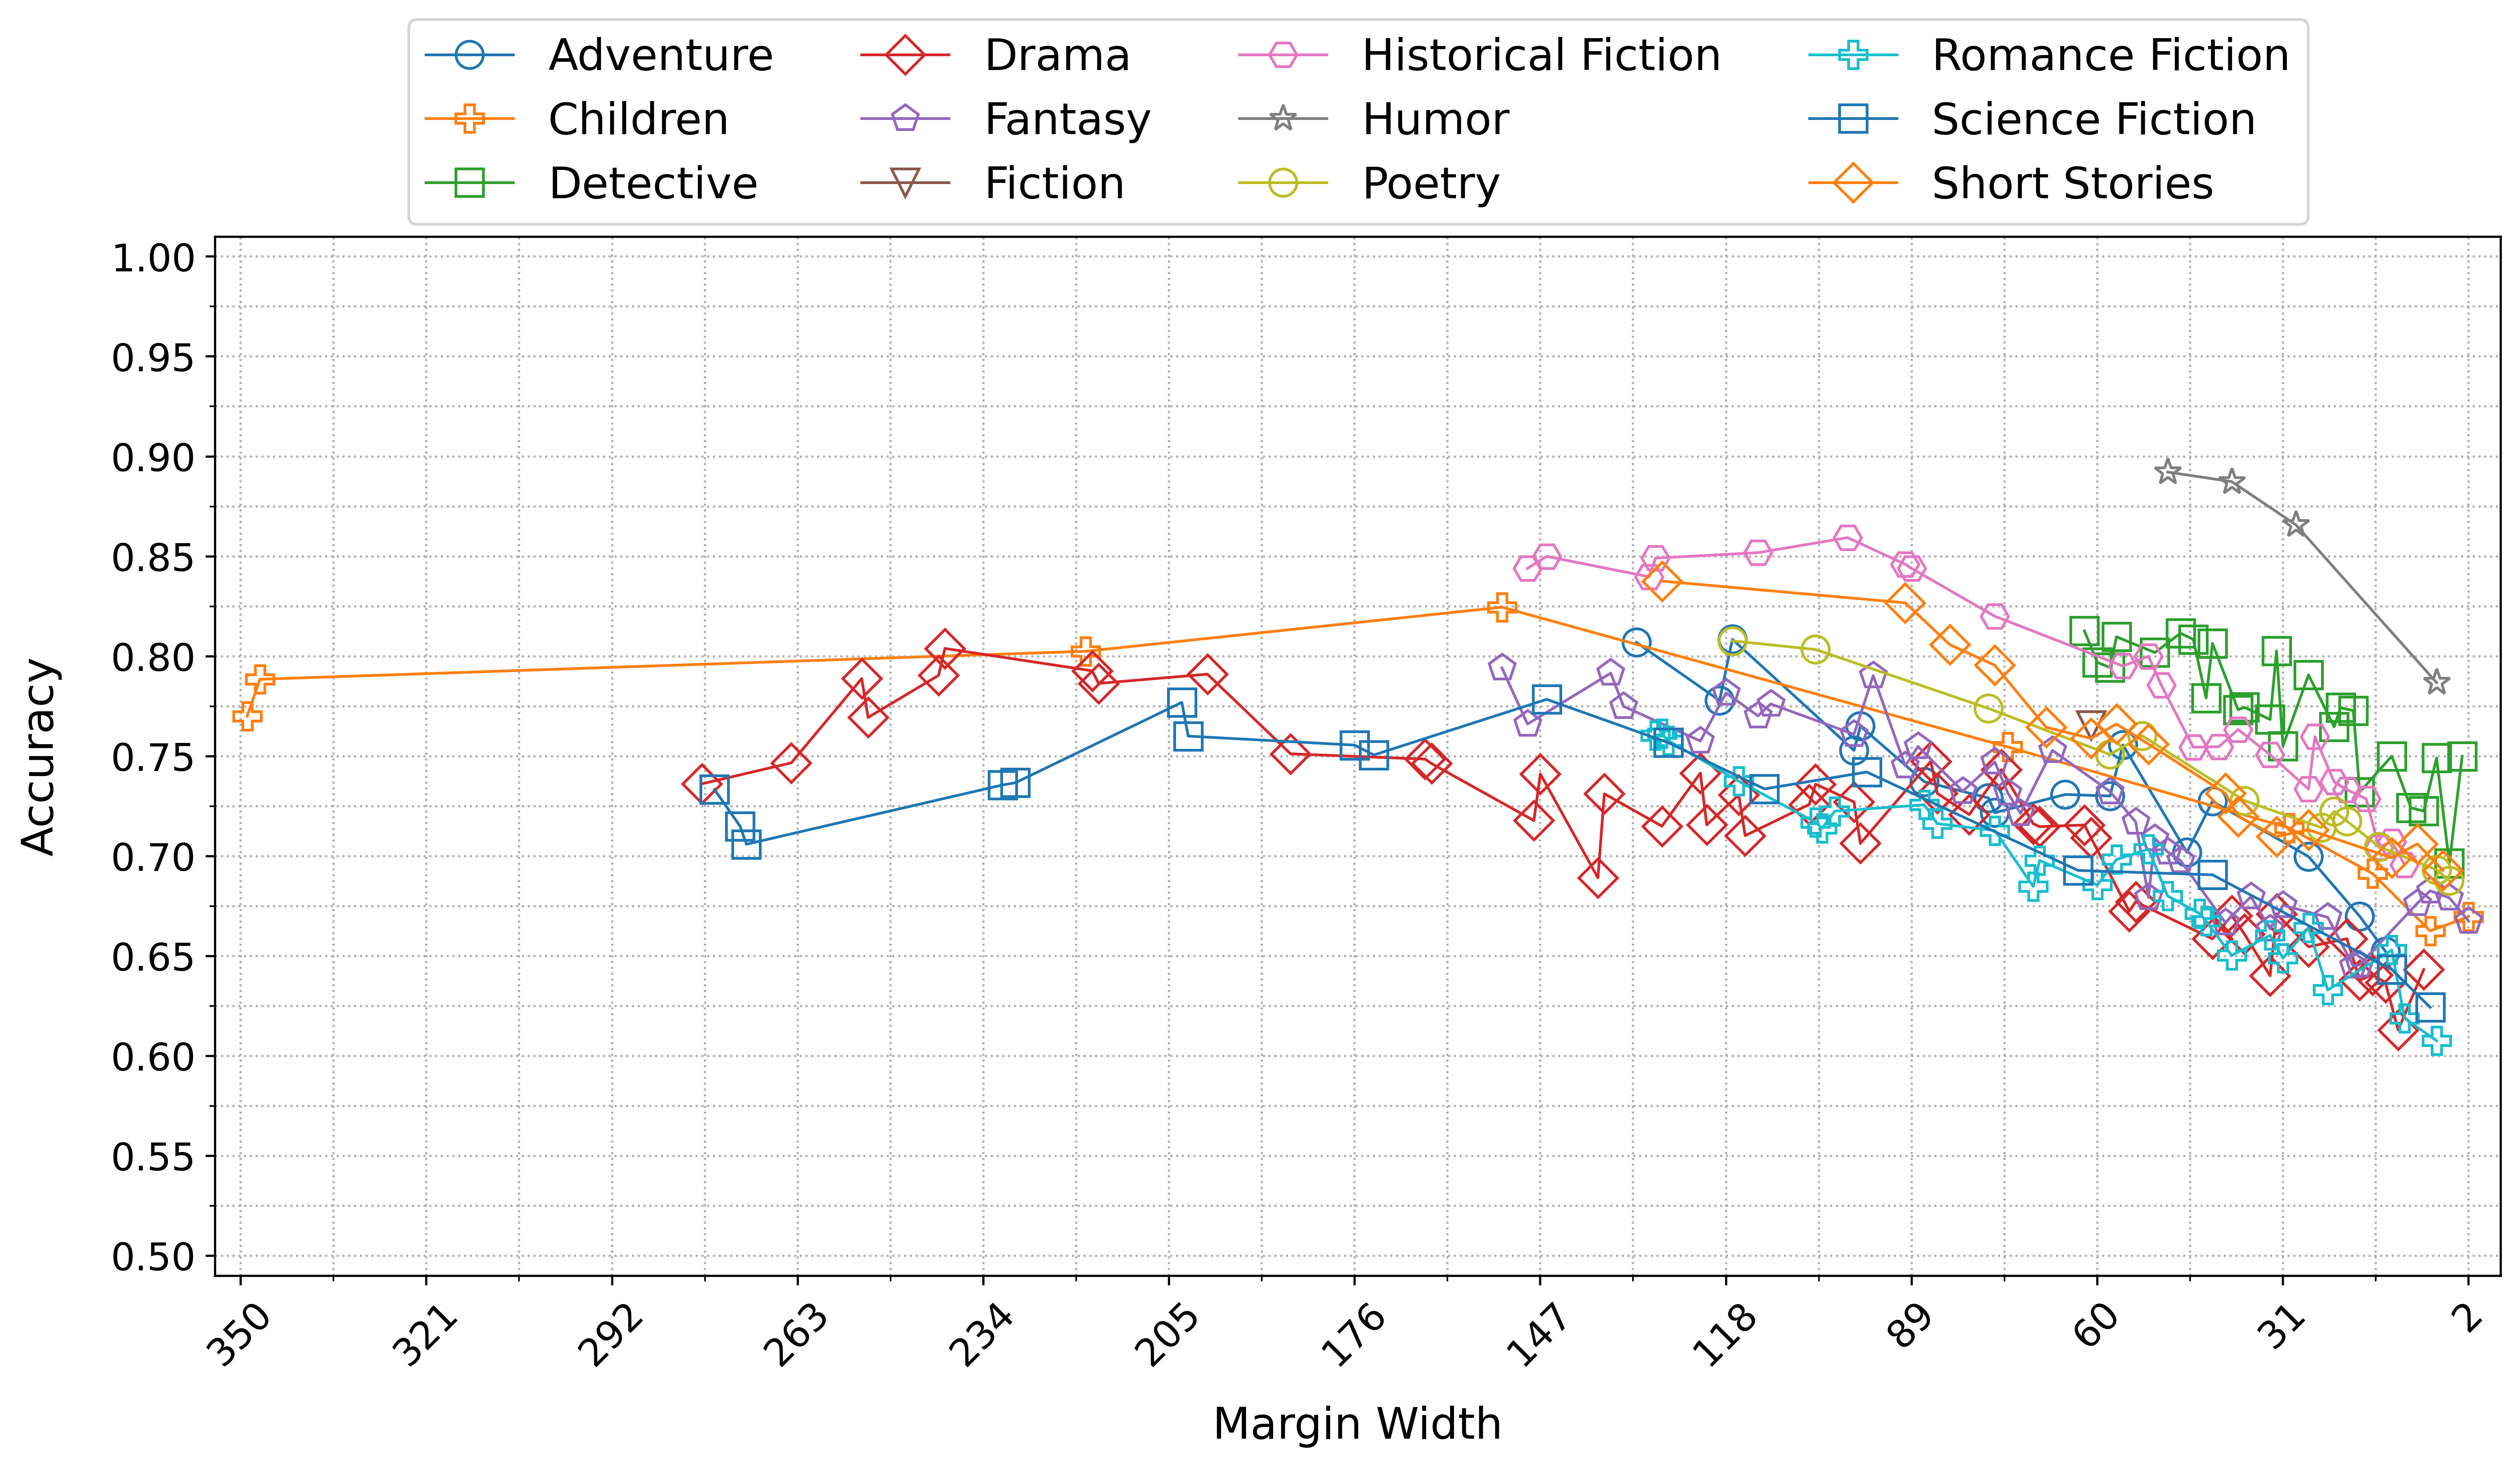
\includegraphics[width=\textwidth]{figures/pngs/roget threshold search by genre.png}
\end{figure*}
% \vspace*{-\baselineskip}

% \vspace*{-\baselineskip}
% \vspace*{-\baselineskip}
\begin{figure*}[!thb]
    \caption{WordNet book success prediction accuracy by genre vs. difference of $\upsilon^-$ and $\upsilon^+$}
    \label{fig:wn threshold search by genre}
    \centering
    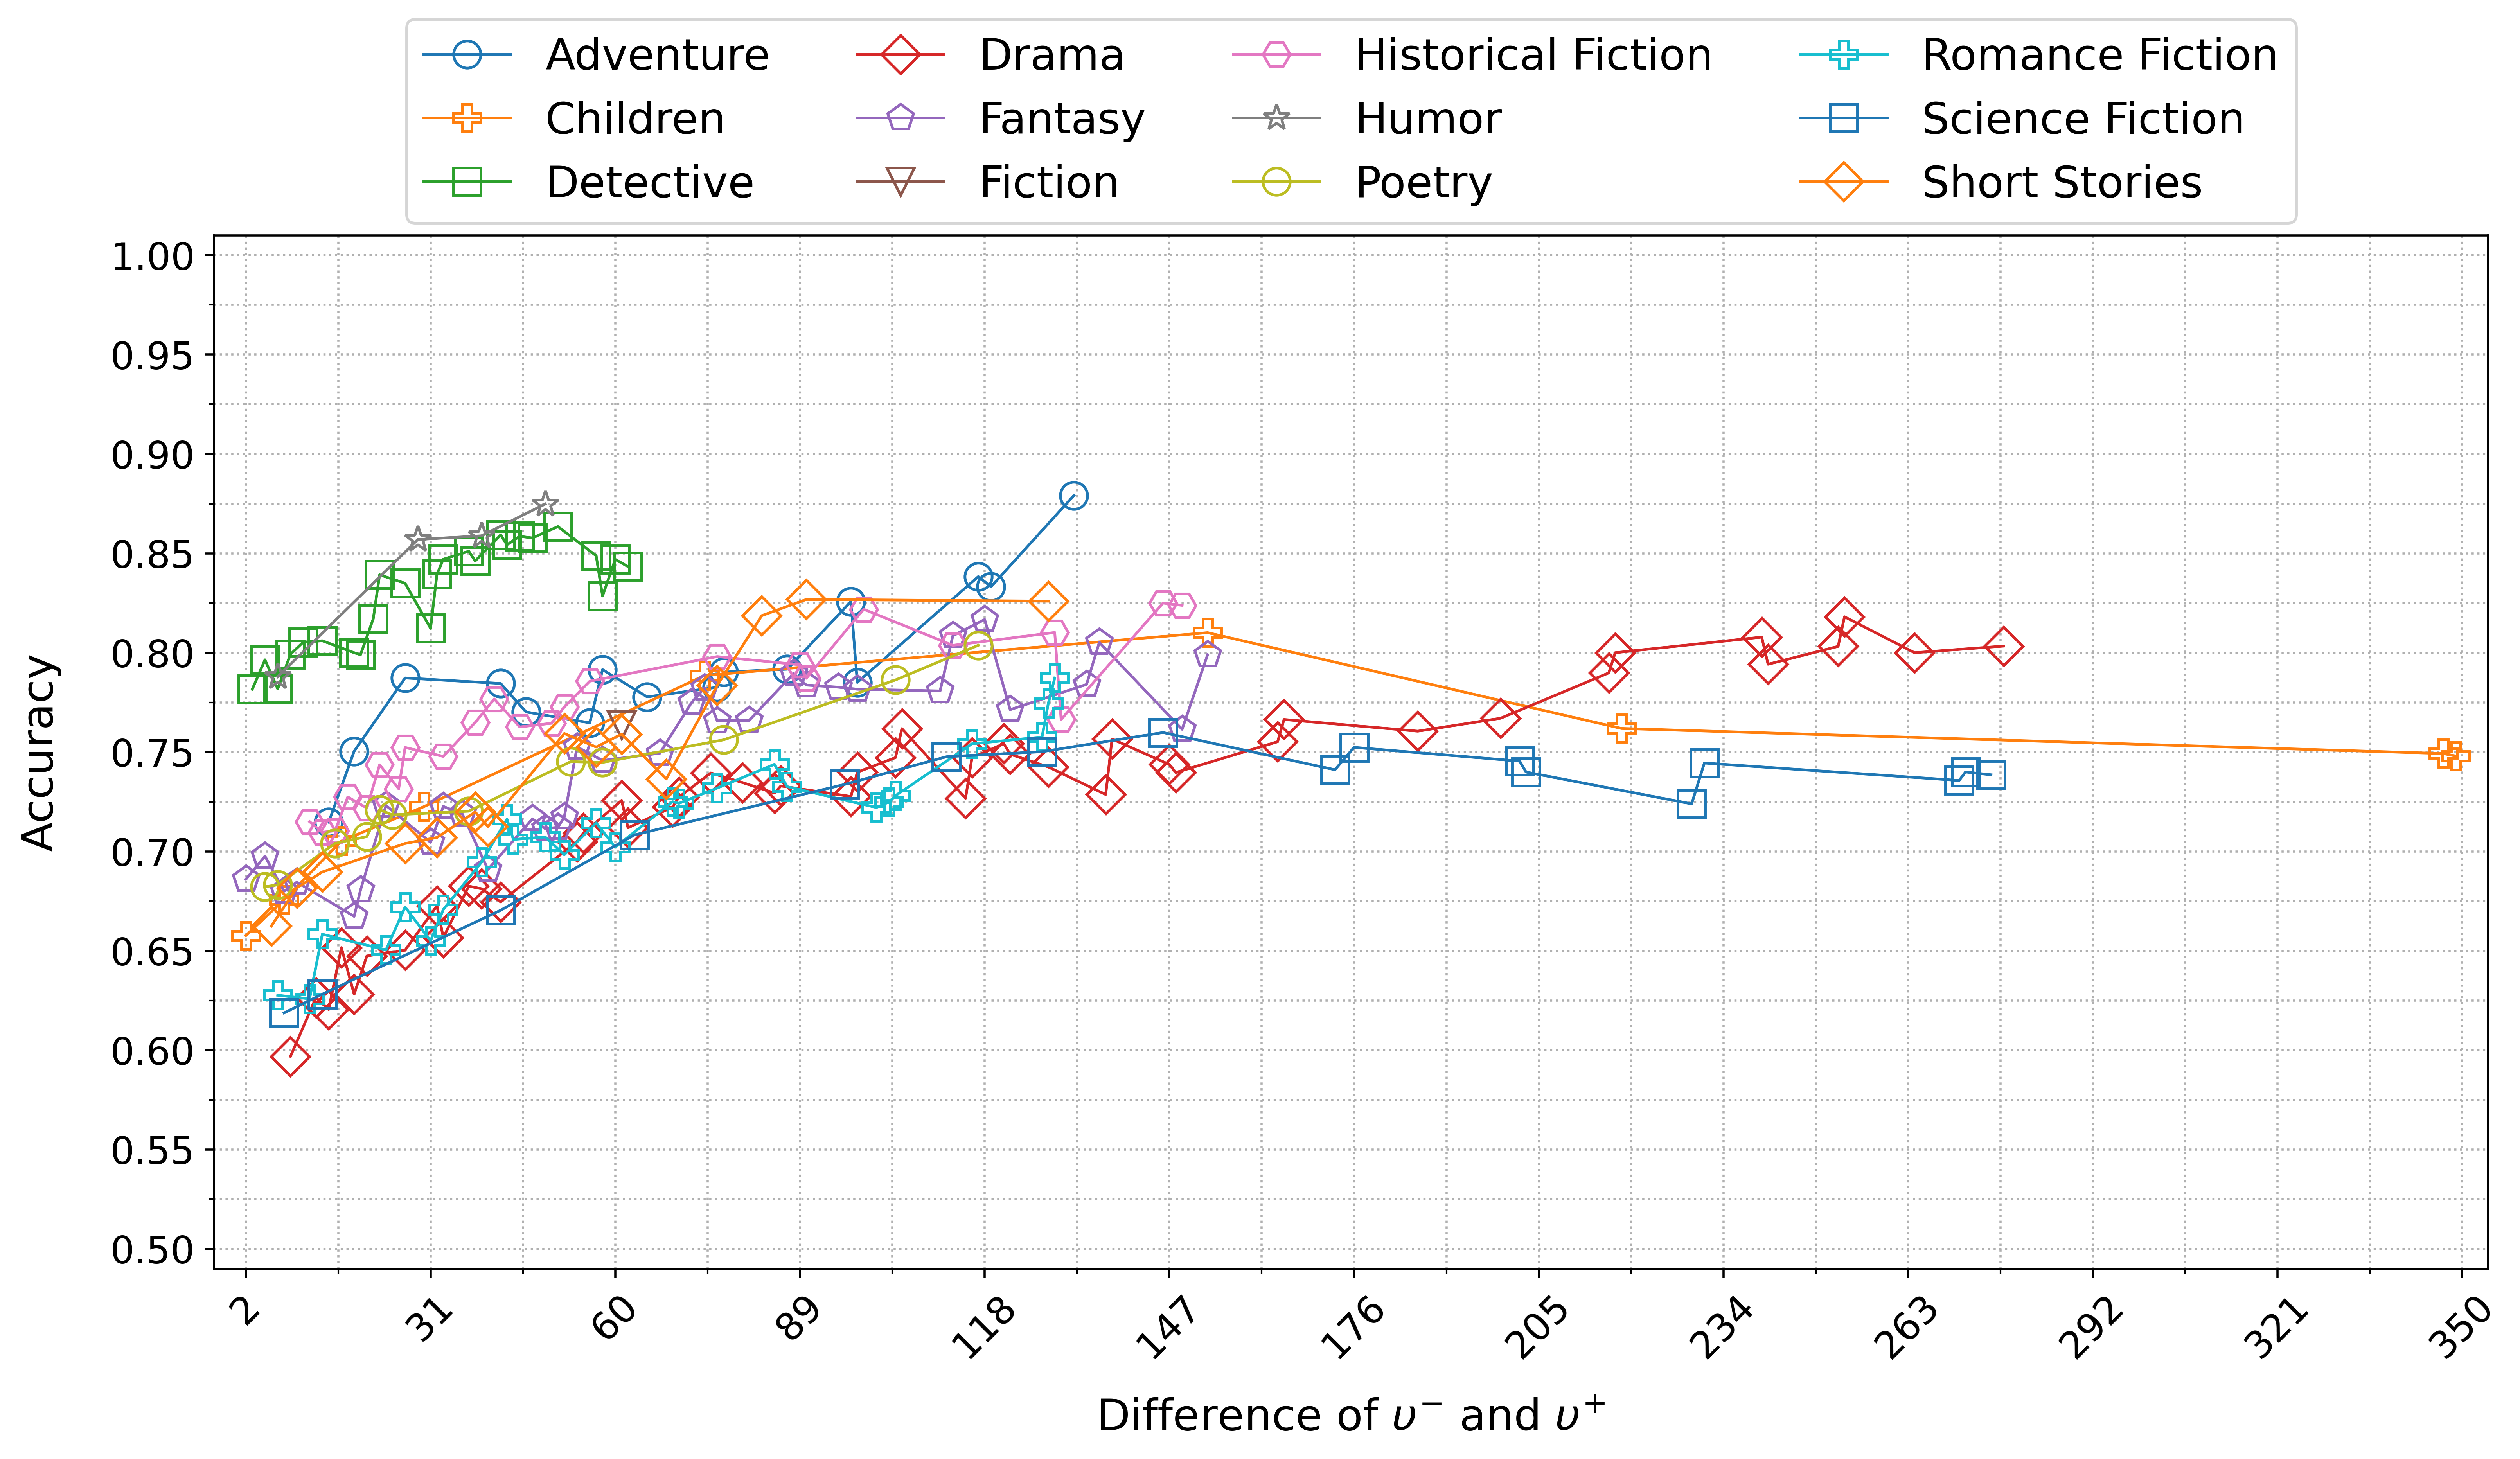
\includegraphics[width=\textwidth]{figures/pngs/wn threshold search by genre.png}
\end{figure*}
% \vspace*{-\baselineskip}

\begin{figure*}[thb]
    \centering
    \caption{Feature reduction process: WordNet success prediction accuracy vs. number of features}
    \label{fig:wn feature reduction}
% \begin{subfigure}{\columnwidth}
    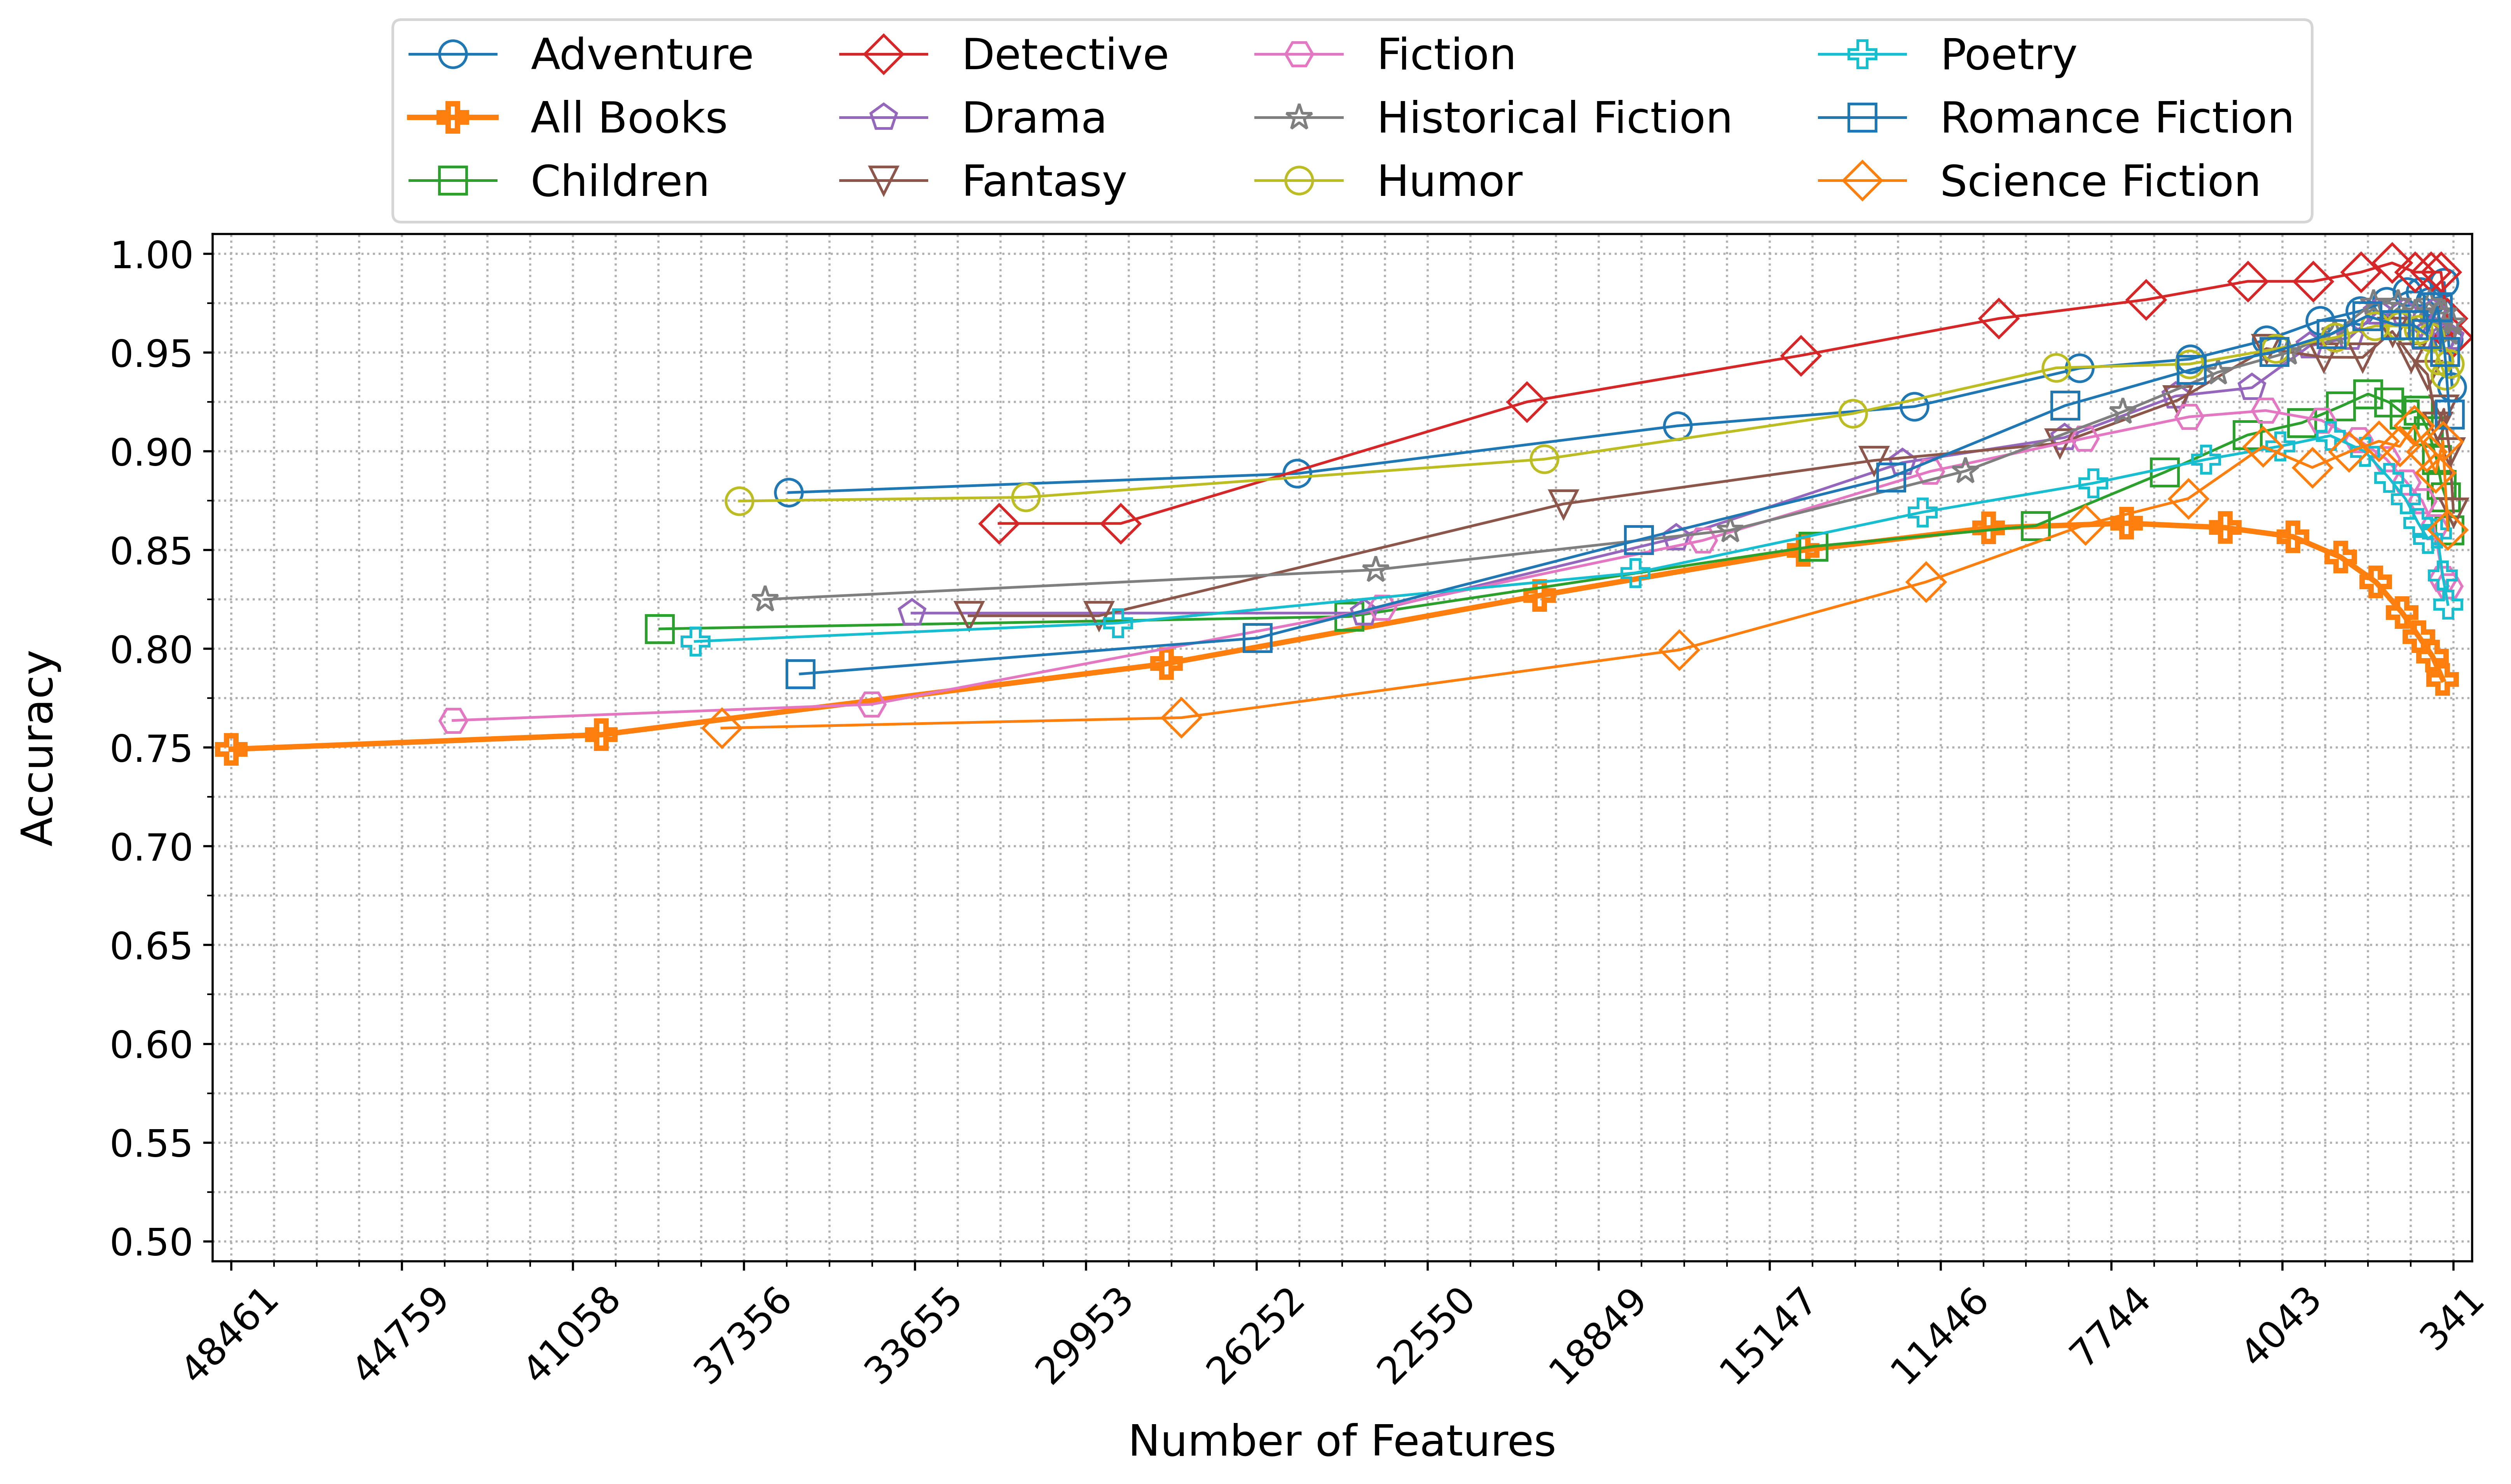
\includegraphics[width=\textwidth]{figures/pngs/wn_feature_reduction_by_genre.png}
    % \par \bigskip
    % 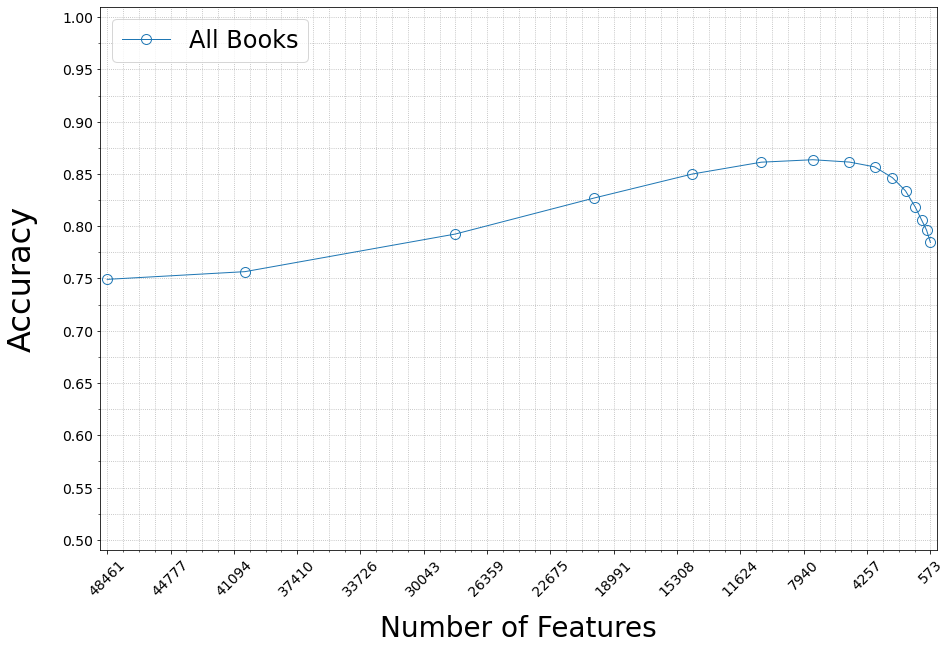
\includegraphics[width=\columnwidth]{figures/pngs/wn_feature_reduction_ALL.png}
% \end{subfigure}
\end{figure*}


\section{Introduction}\label{sec:introduction}

Predicting the success of a novel by analyzing its content is a challenging research problem.
Thousands of new books are published every year, and only a fraction of them achieve wide popularity.
So the prediction of a book success could be exceptionally useful to the publishing industry and enable editors to make better decisions. 
Many factors contribute to a book's success including, but not limited to,
plot, setting, character development, etc.
Additionally, there are some other factors that contribute to a book's popularity that an author and publisher cannot control like the time when the book is published, the author's reputation, and the marketing strategy. 
In this paper, we only focus on the content of the book to predict its popularity. 

%Literary analysis is the practice of dissecting a work of text's to discern deeper meaning, and is therefore ultimately subjective. 
%Readers, publishers, editors, etc. cannot use literary analysis to make empirical conclusions about any work of writing.
%The authors of~\cite{ashok2013} were the first to use statistical stylometry to predict the success of a novel based only on the contents of its first 1,000 sentences, and their work showed very promising results with the best model reaching 84\% accuracy when predicting the success of \textsc{Adventure} books. 

\subsection*{Previous Work}
The authors of~\cite{ashok2013} were the first to use statistical stylometry to predict the success of a novel based only on the contents of its first 1,000 sentences. 
Ashok et al. used stylistic approaches, such as uni-gram, bi-gram, distribution of the parts-of-speech, grammatical rules, constituent tags, and sentiment and connotation values as features with a Linear SVM~\cite{LIB} for the classification task. 
The authors used books from 8 total genres, and they were able to achieve an average accuracy of 75.7\% for across all genres excluding \textsc{Historical Fiction}. 

In~\cite{maharjan_multitask}, Maharajan et al. used a set of hand crafted features in combination with a recurrent neural network and generated feature representation to predict the likelihood of novel success.
The authors of~\cite{maharjan_multitask} obtained an average accuracy of 73.5\% for across 8 genres.
They also performed several experiments, including using all the features used in~\cite{ashok2013}, sentiment concepts~\cite{Senticnet}, different readability metrics, doc2vec~\cite{Doc2Vec} representation of a book, and unaligned word2vec~\cite{Word2Vec} model of the book. 

In a more recent work~\cite{maharjan_emotion}, Maharajan et al. used the flow of the emotions across books for success prediction and obtained an F1-score of 69\%.
They divided the book into chunks, counted the frequency of emotional associations for each word using the NRC emotion lexicon~\cite{NRC}, and then employed a recurrent neural network with an attention mechanism to predict both the genre and the success.

\subsection*{New Work and Improvements}
We discovered various issues with the dataset used in~\cite{ashok2013}\footnote{\url{https://www3.cs.stonybrook.edu/~songfeng/success/}} including, but not limited to its size, contents, and uniformity.
This original dataset is quite small as it only includes the first 1,000 sentences from 800 books split into 8 different genres, which are further split into successful and unsuccessful classes, each having 50 books.
Additionally, many of the files included have less than 1,000 sentences, or contain automatically generated text from Project Gutenberg instead of the text from the proper novel.
Finally, the books included are prelabled with their successful/unsuccessful class, which limits further testing.

Considering these issues, we decided to build upon~\cite{ashok2013}, but made following critical changes:
\begin{itemize}
    \item Built the largest dataset containing a total of 17,962 books.
    %\item Implemented our own preprocessing methods.
    \item Analyzed the \textit{entire} content of each book and employed alternative prediction models.
    \item Introduced our feature reduction method to further improve model performance.
\end{itemize}
This leads to the motivation for this research and subsequent hypothesis.
We believed that we could greatly improve upon the results of~\cite{ashok2013} with a cleaner and more complete dataset.
We hypothesized that there must be at least one model that is both more accurate and more general than uni-gram, and from such a model, we could discover more interesting and revealing qualities that separate successful from non-successful books.
Ultimately, through our improved methodology and larger dataset, our best models achieve over 95\% accuracy for success prediction and identify the thematic elements prioritized by successful novels of a given genre.

\section{Dataset Construction}\label{sec:dataset-construction}

\subsection*{Classification Results}
The prediction accuracy for each model by genre, and each model across all books, both before and after feature reduction are shown in Table~\ref{tab:results by genre} and Table~\ref{tab:results all}, respectively\footnote{All WordNet to Roget models are mapped from WordNet\textsuperscript{R}}.
As illustrated in both settings, the performance of nearly every model improved after we reduced the features with WordNet showing the largest improvement of an average of 11.9\% when reduced by genre and 8.8\% when reduced independent of genre.

The best performing models are indicated in bold in Table~\ref{tab:results by genre} and Table~\ref{tab:results all}.
When predicting novel success by genre, WordNet\textsuperscript{R} and WNRC\textsuperscript{R} show the best results with both models predicting a book's success class at 95.4\%.
WordNet\textsuperscript{R} is most accurate with \textsc{Adventure} books, with an accuracy of 98.5\%, while WNRC\textsuperscript{R} is able to predict the success of \textsc{Historical Fiction} books with 100\% accuracy.
When predicting the success of a book independent of genre, WordNet\textsuperscript{R} remains the most accurate at 86.3\%.

Figure~\ref{fig:wn feature reduction} illustrates the pattern of performance improvement that each model exhibits through the feature reduction process both by genre and independent of genre.
As the number of features is reduced, the average accuracy for success prediction increases until the algorithm finds the best set of features and achieves peak performance.
Then accuracy sharply drops as the feature set is reduced further.
The fact that each model demonstrates such behavior validates the effectiveness of our feature reduction method.

\begin{table}[!t]
    \caption{Accuracy (\%) of classification results for all books, before/after feature reduction}
    \label{tab:results all}
    \begin{tabular}{c|c|c}
        % \hline
        \centering
        \textsc{Model} & \textsc{Accuracy} & \textsc{Accuracy\textsuperscript{R}} \\
        \hline
        Unigram & 68.7 & \textbf{70.3} \\
        % Unigram\textsuperscript{R} & 86.2}\\
        % \hline
        % Bigram & & & & & & & & & & & & & \\
        % Bigram\textsuperscript{R} & & & & & & & & & & & & & \\
        \hline
        POS & 67.4%42330 
        & 67.4%42332 \\
        \\
        % POS\textsuperscript{R} & 73.0} \\
        \hline
        Roget & 73.5 & 74.8 \\
        % Roget\textsuperscript{R} & 81.8} \\
        \hline
        WordNet & 74.9 & \textbf{86.3} \\
        % WordNet\textsuperscript{R} & 92.6} \\
        \hline
        WNRC & 76.4 & \textbf{77.4} \\
        \hline
        WNRT & 69.5 & 69.5 \\
        % \hline
        % \hline
        % Average & ? & ?} \\
        % Average\textsuperscript{R} & 83.4} \\
        % \hline
        % $\Gamma$ & & & & & & & & & & & & & \\
        % $\Gamma^R$ & & & & & & & & & & & & & \\
        % \hline
        % $\Gamma^G$ & & & & & & & & & & & & & \\
        % $\Gamma^{G^R}$ & & & & & & & & & & & & & \\
        % \hline
        % $\gamma$ & & & & & & & & & & & & & \\
        % $\gamma^R$ & & & & & & & & & & & & & \\
        % \hline
        % $\gamma^G$ & & & & & & & & & & & & & \\
        % $\gamma^{G^R}$ & & & & & & & & & & & & & \\
        \hline
    \end{tabular}
\end{table}

\subsection*{Interpreting Book Success}\label{subsec:int book success}
While our reduced WordNet model displays excellent performance in both test settings (by genre and independent of genre), the resulting feature sets are not self-explanatory.
In other words, the Synsets that the model deems most important do not necessarily highlight some interesting aspect of successful books, expected or otherwise.
This is where \textit{Roget's Thesaurus} proves most valuable.

We figured that if we looked up the Roget Theme of each WordNet Synset that we would find that the successful and unsuccessful books prioritize different Themes.
This was possible due to the similarity in the structure of WordNet and \textit{Roget's Thesaurus} as explained in the \textbf{Methodology} section above.
With this hypothesis in mind, we mapped the reduced WordNet model to a new Roget model by first looking up the Roget Category of each Synset from the reduced WordNet feature set, and then summing the frequencies in each group of Sysnets.
Then, as we did with each previous model, we reduced the new WordNet-to-Roget-Category (WNRC) model.
From the WNRC\textsuperscript{R} model we mapped again, this time from Roget Categories to the 23 Roget Themes, which produced the WordNet-to-Roget-Themes (WNRT) model.

We did not expect the performance of the WNRC model, since it was conceived strictly as an intermediary map between WordNet and Roget Themes. 
WNRC produced the highest baseline results of all the models used in our experiments with 89.5\% average accuracy by genre, and was able to perfectly predict the success classification of \textsc{Historical Fiction} novels.
Furthermore, WNRC\textsuperscript{R} accurately predicts success classification per genre at an average rate of 95.4\%, tying it with WordNet\textsuperscript{R} as the best performing models we tested.
What's impressive about the accuracy of WNRC\textsuperscript{R} when compared to that of WordNet\textsuperscript{R} is the large difference in number of features used in each model as shown in Table~\ref{tab:wn vs wnrc features}.

\begin{table}[t]
    \caption{Number of features before/after reduction for WordNet, WNRC, and WNRT}
    \label{tab:wn vs wnrc features}
    \begin{tabular}{l|r|r|r}
        % \hline
        % \multirow{2}{*}{Genre} & \multicolumn{3}{|c}{Number of Features} \\
        % \cline{2-4}
        % & WordNet & WNRC & WNRS \\
        % \hline
        %%
        %%%%
        % UPDATE ALL %%%
        %%%%
        \centering
        \textsc{Genre} & \textsc{WordNet} & \textsc{WNRC} & \textsc{WNRT} \\
        \hline
        Adventure & 36,390 & 425 & 22 \\
        Adventure\textsuperscript{R} & 540 & 149 & 17 \\
        \hline
        Children & 39,179 & 864 & 23 \\
        Children\textsuperscript{R} & 2,117 & 210 & 14 \\
        \hline
        Detective & 31,833 & 840 & 21 \\
        Detective\textsuperscript{R} & 1,670 & 272 & 9 \\
        \hline
        Drama & 33,718 & 812 & 23 \\
        Drama\textsuperscript{R} & 1,996 & 333 & 3 \\
        \hline
        Fantasy & 32,483 & 779 & 21 \\
        Fantasy\textsuperscript{R} & 1,665 & 192 & 12 \\
        \hline
        Fiction & 43,655 & 963 & 23 \\
        Fiction\textsuperscript{R} & 4,407 & 403 & 10 \\
        \hline
        Hist. Fict. & 36,902 & 815 & 22 \\
        Hist. Fict.\textsuperscript{R} & 864 & 198 & 14 \\
        \hline
        Humor & 37,457 & 822 & 22 \\
        Humor\textsuperscript{R} & 1,493 & 324 & 7 \\
        \hline
        Poetry & 38,412 & 872 & 23 \\
        Poetry\textsuperscript{R} & 3,004 & 243 & 7 \\
        \hline
        Romance & 36,137 & 451 & 23 \\
        Romance\textsuperscript{R} & 688 & 129 & 12 \\
        \hline
        Sci-Fi & 37,835 & 617 & 23 \\
        Sci-Fi\textsuperscript{R} & 1,190 & 225 & 6 \\
        \hline
        Short & 36,912 & 964 & 22 \\
        Short\textsuperscript{R} & 3,769 & 217 & 16 \\
        \hline
        All & 48,461 & 1,001 & 23 \\
        All\textsuperscript{R} & 7,415 & 374 & 23 \\
        \hline
    \end{tabular}
\end{table}

With such impressive results from WNRC\textsuperscript{R}, we expected WNRT and WNRT\textsuperscript{R} to follow suit despite learning with a feature set of at most 23 features.
WNRT\textsuperscript{R} achieves an average accuracy of 83.7\% learning from an average of only 10 features. 
While the performance of WNRT\textsuperscript{R} is impressive given the few number of features it requires, the purpose of WNRT\textsuperscript{R} was not to outperform WordNet\textsuperscript{R} or WNRC\textsuperscript{R}.
As previously state, the motivation for the construction of WNRT was strictly to find a common thread between successful novels in each genre.
That said, the decent performance of the WNRT\textsuperscript{R} model does support the reasoning behind its conception, and provide further evidence that WordNet\textsuperscript{R} and WNRC\textsuperscript{R} are general models that can reveal underlying characteristics of successful books.

\begin{table*}[!t]
    \caption{Top 5 most important themes for classifying \textsc{Children} novels and successful/unsuccessful thematic words}
    \label{tab:child themes}
    \begin{tabular}{l|ll}
        \hline
        \centering
        \multirow{2}{*}{\textsc{Theme}} & \multicolumn{2}{c}{\textsc{Words}} \\
        \cline{2-3}
        & \multicolumn{1}{c|}{Successful} & \multicolumn{1}{c}{Unsuccessful} \\
        \hline
        Affections & enthusiastic, lively, tenderness & inactive, sluggish, dull \\
        Communication of Ideas & secret, untruth, language & school, grammar, taciturnity \\
        Formation of Ideas & incredulity, impossibility, curiosity & dissent, sanity, memory \\
        Moral & gluttony, impurity, selfishness & punishment, virtue, duty \\
        Personal & expecting, blemish, hopelessness & aggravation, dejection, dullness \\
        \hline
    \end{tabular}
\end{table*}

Additionally, WNRT does not improve performance after feature reduction when classifying independent of genre.
This outcome also supports our original hypothesis as it shows that the model requires each of the 23 Roget Themes in order to make the most accurate prediction.
The lack of improvement in WNRT\textsuperscript{R} when predicting success class independent of genre also demonstrates the relationship between a novel's genre and its prioritization of certain Themes.

\subsection*{Successful Lexical Choices}\label{subsec:successful lexical choices}

After mapping the resulting feature weights of our WordNet\textsuperscript{R} model to Roget Themes, we were able to highlight the most important Themes when classifying the success of a novel given its genre.
Table~\ref{tab:child themes} gives the most important themes in predicting the success of \textsc{Children's} novels and the successful and unsuccessful semantic word groups within those themes.
These results clearly identify words associated with "school" and "grammar" as key contributors to unsuccessful \textsc{Children's} novels, while words like "secret," "enthusiastic," and "selfishness" contribute to successful \textsc{Children's} novels.

The indicated Themes align with intuitive expectations for \textsc{Children's} books, especially the presence of \textsc{Formation of Ideas} and \textsc{Moral}.
To verify these results, we looked at the most downloaded \textsc{Children's} book, \textit{Little Women}.
We ranked each book in the \textsc{Children's} genre according to the frequency of each prioritized Themes listed in Table~\ref{tab:little women}.
Then, we looked to see where \textit{Little Women} ranked for each of the Themes.
\textit{Little Women}'s use of the top Themes matches up as expected, as it ranks in the top three for four of the five most important Themes, and eighth for the fifth as shown in Table~\ref{tab:little women}.
The opposite is true for the least downloaded books, which all rank at the bottom for use of the most important Themes.

% \begin{figure}[t]
    \centering
    \caption{\textit{Little Women} by Louisa May Alcott}
    \label{fig:little women cover}
    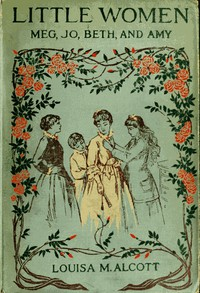
\includegraphics[width=0.25\columnwidth]{figures/pngs/little women cover.jpg}
\end{figure}

\begin{table}[h]
    \caption{Ranking the use of the most important \textsc{Children's} themes for \#1 downloaded \textsc{Children's} book, \textit{Little Women} relative to other \textsc{Children's} books in the dataset}
    \label{tab:little women}
    \begin{tabular}{l|r}
        \hline
        \centering
        \textsc{Theme} & \textsc{Rank} \\
        \hline
        Communication of Ideas & 2 \\
        Formation of Ideas & 2 \\
        Personal & 2 \\
        Moral & 3 \\
        Affections & 8 \\
        \hline
    \end{tabular}
\end{table}

Our Thematic observations hold true for each genre, but there is not one theme shared by all 12 genres.%, and Table~\ref{tab:theme counts} shows the distribution of Theme prioritization across all 12 genres.
This adheres to the observation we made about the WNRT and its lack of improvement after feature reduction for predicting success of all books.

\begin{table*}[!t]
    \caption{Accuracy (\%) of classification results by genre, with/without feature reduction (R) (\textit{best performance in bold})}
    \label{tab:results by genre}
    \begin{tabular}{c|cccccccccccc|c}
        \hline
        \centering
        \multirow{2}{*}{\textsc{Model}} & \multicolumn{12}{|c|}{\textsc{Genre}} & \multirow{2}{*}{\textsc{Avg}} \\
        \cline{2-13}
        & Adv. & Child. & Detective & Drama & Fantasy & Fiction & Hist. Fict. & Humor & Poetry & Romance & Sci-Fi & Short & \\
        \hline
        Unigram & 77.0 & 77.2 & 84.2 & 74.7 & 78.4 & 70.2 & 76.8 & 84.2 & 74.0 & 73.4 & 76.0 & 69.6 & 76.3 \\
        Unigram\textsuperscript{R} & 79.1 & 82.7 & 86.7 & 78.3 & 80.4 & 75.6 & 80.4 & 88.3 & 79.0 & 77.9 & 81.3 & 78.2 & 80.6 \\
        % \hline
        % Bigram & & & & & & & & & & & & & \\
        % Bigram\textsuperscript{R} & & & & & & & & & & & & & \\
        \hline
        POS & 79.7 & 76.4 & 77.2 & 69.1 & 75.4 & 73.7 & 84.9 & 86.7 & 77.6 & 72.9 & 74.9 & 79.3 & 77.3 \\
        POS\textsuperscript{R} & 80.2 & 77.9 & 79.3 & 70.0 & 77.4 & 74.3 & 84.9 & 87.3 & 77.6 & 75.6 & 75.5 & 80.8 & 78.4 \\
        \hline
        Roget & 80.9 & 82.5 & 81.3 & 80.4 & 79.4 & 76.6 & 85.9 & 89.2 & 80.8 & 76.1 & 77.8 & 83.8 & 81.2 \\
        Roget\textsuperscript{R} & 87.2 & 88.5 & 94.9 & 85.9 & 92.0 & 79.9 & 87.8 & 91.5 & 84.5 & 85.2 & 82.1 & 90.5 & 87.5 \\
        \hline
        WordNet & 87.9 & 81.0 & 86.3 & 81.8 & 81.7 & 76.4 & 82.5 & 87.5 & 80.4 & 78.7 & 76.0 & 82.7 & 81.9 \\
        WordNet\textsuperscript{R} & \textbf{98.5} & 92.9 & \textbf{99.5} & 97.0 & 96.1 & \textbf{92.1} & 97.5 & 96.3 & \textbf{90.8} & 97.3 & 91.3 & \textbf{95.4} & \textbf{95.4} \\
        \hline
        WNRC & 94.3 & 89.8 & 92.4 & 92.8 & 86.0 & 82.1 & 97.0 & 94.4 & 82.4 & 91.9 & 84.9 & 86.4 & 89.5 \\
        WNRC\textsuperscript{R} & \textbf{98.5} & \textbf{93.7} & \textbf{99.5} & \textbf{98.3} & \textbf{96.9} & 85.9 & \textbf{100.0} & \textbf{97.3} & 87.5 & \textbf{97.7} & \textbf{93.9} & \textbf{95.4} & \textbf{95.4} \\
        \hline
        WNRT & 80.7 & 77.7 & 82.5 & 82.3 & 73.8 & 74.0 & 93.0 & 87.7 & 77.6 & 85.5 & 78.6 & 84.5 & 81.5 \\
        WNRT\textsuperscript{R} & 90.8 & 78.3 & 87.7 & 84.0 & 79.5 & 74.8 & 92.0 & 88.6 & 79.3 & 83.7 & 81.5 & 84.3 & 83.7 \\
        % \hline
        % \hline
        % \textsc{Average} & 84.4 & 80.6 & 84.6 & 79.4 & 80.0 & 75.5 & 86.5 & 88.3 & 78.9 & 78.6 & 78.1 & 81.1 & 81.3 \\
        % \textsc{Average\textsuperscript{R}} & 89.1 & 85.7 & 91.3 & 85.6 & 87.0 & 80.4 & 90.4 & 91.6 & 83.1 & 86.2 & 84.3 & 87.4 & 86.8 \\
        % \hline
        % $\Gamma$ & & & & & & & & & & & & & \\
        % $\Gamma^R$ & & & & & & & & & & & & & \\
        % \hline
        % $\Gamma^G$ & & & & & & & & & & & & & \\
        % $\Gamma^{G^R}$ & & & & & & & & & & & & & \\
        % \hline
        % $\gamma$ & & & & & & & & & & & & & \\
        % $\gamma^R$ & & & & & & & & & & & & & \\
        % \hline
        % $\gamma^G$ & & & & & & & & & & & & & \\
        % $\gamma^{G^R}$ & & & & & & & & & & & & & \\
        \hline
    \end{tabular}
\end{table*}

\section{Methodology}\label{sec:methodology}

\subsection*{Classification Results}
The prediction accuracy for each model by genre, and each model across all books, both before and after feature reduction are shown in Table~\ref{tab:results by genre} and Table~\ref{tab:results all}, respectively\footnote{All WordNet to Roget models are mapped from WordNet\textsuperscript{R}}.
As illustrated in both settings, the performance of nearly every model improved after we reduced the features with WordNet showing the largest improvement of an average of 11.9\% when reduced by genre and 8.8\% when reduced independent of genre.

The best performing models are indicated in bold in Table~\ref{tab:results by genre} and Table~\ref{tab:results all}.
When predicting novel success by genre, WordNet\textsuperscript{R} and WNRC\textsuperscript{R} show the best results with both models predicting a book's success class at 95.4\%.
WordNet\textsuperscript{R} is most accurate with \textsc{Adventure} books, with an accuracy of 98.5\%, while WNRC\textsuperscript{R} is able to predict the success of \textsc{Historical Fiction} books with 100\% accuracy.
When predicting the success of a book independent of genre, WordNet\textsuperscript{R} remains the most accurate at 86.3\%.

Figure~\ref{fig:wn feature reduction} illustrates the pattern of performance improvement that each model exhibits through the feature reduction process both by genre and independent of genre.
As the number of features is reduced, the average accuracy for success prediction increases until the algorithm finds the best set of features and achieves peak performance.
Then accuracy sharply drops as the feature set is reduced further.
The fact that each model demonstrates such behavior validates the effectiveness of our feature reduction method.

\begin{table}[!t]
    \caption{Accuracy (\%) of classification results for all books, before/after feature reduction}
    \label{tab:results all}
    \begin{tabular}{c|c|c}
        % \hline
        \centering
        \textsc{Model} & \textsc{Accuracy} & \textsc{Accuracy\textsuperscript{R}} \\
        \hline
        Unigram & 68.7 & \textbf{70.3} \\
        % Unigram\textsuperscript{R} & 86.2}\\
        % \hline
        % Bigram & & & & & & & & & & & & & \\
        % Bigram\textsuperscript{R} & & & & & & & & & & & & & \\
        \hline
        POS & 67.4%42330 
        & 67.4%42332 \\
        \\
        % POS\textsuperscript{R} & 73.0} \\
        \hline
        Roget & 73.5 & 74.8 \\
        % Roget\textsuperscript{R} & 81.8} \\
        \hline
        WordNet & 74.9 & \textbf{86.3} \\
        % WordNet\textsuperscript{R} & 92.6} \\
        \hline
        WNRC & 76.4 & \textbf{77.4} \\
        \hline
        WNRT & 69.5 & 69.5 \\
        % \hline
        % \hline
        % Average & ? & ?} \\
        % Average\textsuperscript{R} & 83.4} \\
        % \hline
        % $\Gamma$ & & & & & & & & & & & & & \\
        % $\Gamma^R$ & & & & & & & & & & & & & \\
        % \hline
        % $\Gamma^G$ & & & & & & & & & & & & & \\
        % $\Gamma^{G^R}$ & & & & & & & & & & & & & \\
        % \hline
        % $\gamma$ & & & & & & & & & & & & & \\
        % $\gamma^R$ & & & & & & & & & & & & & \\
        % \hline
        % $\gamma^G$ & & & & & & & & & & & & & \\
        % $\gamma^{G^R}$ & & & & & & & & & & & & & \\
        \hline
    \end{tabular}
\end{table}

\subsection*{Interpreting Book Success}\label{subsec:int book success}
While our reduced WordNet model displays excellent performance in both test settings (by genre and independent of genre), the resulting feature sets are not self-explanatory.
In other words, the Synsets that the model deems most important do not necessarily highlight some interesting aspect of successful books, expected or otherwise.
This is where \textit{Roget's Thesaurus} proves most valuable.

We figured that if we looked up the Roget Theme of each WordNet Synset that we would find that the successful and unsuccessful books prioritize different Themes.
This was possible due to the similarity in the structure of WordNet and \textit{Roget's Thesaurus} as explained in the \textbf{Methodology} section above.
With this hypothesis in mind, we mapped the reduced WordNet model to a new Roget model by first looking up the Roget Category of each Synset from the reduced WordNet feature set, and then summing the frequencies in each group of Sysnets.
Then, as we did with each previous model, we reduced the new WordNet-to-Roget-Category (WNRC) model.
From the WNRC\textsuperscript{R} model we mapped again, this time from Roget Categories to the 23 Roget Themes, which produced the WordNet-to-Roget-Themes (WNRT) model.

We did not expect the performance of the WNRC model, since it was conceived strictly as an intermediary map between WordNet and Roget Themes. 
WNRC produced the highest baseline results of all the models used in our experiments with 89.5\% average accuracy by genre, and was able to perfectly predict the success classification of \textsc{Historical Fiction} novels.
Furthermore, WNRC\textsuperscript{R} accurately predicts success classification per genre at an average rate of 95.4\%, tying it with WordNet\textsuperscript{R} as the best performing models we tested.
What's impressive about the accuracy of WNRC\textsuperscript{R} when compared to that of WordNet\textsuperscript{R} is the large difference in number of features used in each model as shown in Table~\ref{tab:wn vs wnrc features}.

\begin{table}[t]
    \caption{Number of features before/after reduction for WordNet, WNRC, and WNRT}
    \label{tab:wn vs wnrc features}
    \begin{tabular}{l|r|r|r}
        % \hline
        % \multirow{2}{*}{Genre} & \multicolumn{3}{|c}{Number of Features} \\
        % \cline{2-4}
        % & WordNet & WNRC & WNRS \\
        % \hline
        %%
        %%%%
        % UPDATE ALL %%%
        %%%%
        \centering
        \textsc{Genre} & \textsc{WordNet} & \textsc{WNRC} & \textsc{WNRT} \\
        \hline
        Adventure & 36,390 & 425 & 22 \\
        Adventure\textsuperscript{R} & 540 & 149 & 17 \\
        \hline
        Children & 39,179 & 864 & 23 \\
        Children\textsuperscript{R} & 2,117 & 210 & 14 \\
        \hline
        Detective & 31,833 & 840 & 21 \\
        Detective\textsuperscript{R} & 1,670 & 272 & 9 \\
        \hline
        Drama & 33,718 & 812 & 23 \\
        Drama\textsuperscript{R} & 1,996 & 333 & 3 \\
        \hline
        Fantasy & 32,483 & 779 & 21 \\
        Fantasy\textsuperscript{R} & 1,665 & 192 & 12 \\
        \hline
        Fiction & 43,655 & 963 & 23 \\
        Fiction\textsuperscript{R} & 4,407 & 403 & 10 \\
        \hline
        Hist. Fict. & 36,902 & 815 & 22 \\
        Hist. Fict.\textsuperscript{R} & 864 & 198 & 14 \\
        \hline
        Humor & 37,457 & 822 & 22 \\
        Humor\textsuperscript{R} & 1,493 & 324 & 7 \\
        \hline
        Poetry & 38,412 & 872 & 23 \\
        Poetry\textsuperscript{R} & 3,004 & 243 & 7 \\
        \hline
        Romance & 36,137 & 451 & 23 \\
        Romance\textsuperscript{R} & 688 & 129 & 12 \\
        \hline
        Sci-Fi & 37,835 & 617 & 23 \\
        Sci-Fi\textsuperscript{R} & 1,190 & 225 & 6 \\
        \hline
        Short & 36,912 & 964 & 22 \\
        Short\textsuperscript{R} & 3,769 & 217 & 16 \\
        \hline
        All & 48,461 & 1,001 & 23 \\
        All\textsuperscript{R} & 7,415 & 374 & 23 \\
        \hline
    \end{tabular}
\end{table}

With such impressive results from WNRC\textsuperscript{R}, we expected WNRT and WNRT\textsuperscript{R} to follow suit despite learning with a feature set of at most 23 features.
WNRT\textsuperscript{R} achieves an average accuracy of 83.7\% learning from an average of only 10 features. 
While the performance of WNRT\textsuperscript{R} is impressive given the few number of features it requires, the purpose of WNRT\textsuperscript{R} was not to outperform WordNet\textsuperscript{R} or WNRC\textsuperscript{R}.
As previously state, the motivation for the construction of WNRT was strictly to find a common thread between successful novels in each genre.
That said, the decent performance of the WNRT\textsuperscript{R} model does support the reasoning behind its conception, and provide further evidence that WordNet\textsuperscript{R} and WNRC\textsuperscript{R} are general models that can reveal underlying characteristics of successful books.

\begin{table*}[!t]
    \caption{Top 5 most important themes for classifying \textsc{Children} novels and successful/unsuccessful thematic words}
    \label{tab:child themes}
    \begin{tabular}{l|ll}
        \hline
        \centering
        \multirow{2}{*}{\textsc{Theme}} & \multicolumn{2}{c}{\textsc{Words}} \\
        \cline{2-3}
        & \multicolumn{1}{c|}{Successful} & \multicolumn{1}{c}{Unsuccessful} \\
        \hline
        Affections & enthusiastic, lively, tenderness & inactive, sluggish, dull \\
        Communication of Ideas & secret, untruth, language & school, grammar, taciturnity \\
        Formation of Ideas & incredulity, impossibility, curiosity & dissent, sanity, memory \\
        Moral & gluttony, impurity, selfishness & punishment, virtue, duty \\
        Personal & expecting, blemish, hopelessness & aggravation, dejection, dullness \\
        \hline
    \end{tabular}
\end{table*}

Additionally, WNRT does not improve performance after feature reduction when classifying independent of genre.
This outcome also supports our original hypothesis as it shows that the model requires each of the 23 Roget Themes in order to make the most accurate prediction.
The lack of improvement in WNRT\textsuperscript{R} when predicting success class independent of genre also demonstrates the relationship between a novel's genre and its prioritization of certain Themes.

\subsection*{Successful Lexical Choices}\label{subsec:successful lexical choices}

After mapping the resulting feature weights of our WordNet\textsuperscript{R} model to Roget Themes, we were able to highlight the most important Themes when classifying the success of a novel given its genre.
Table~\ref{tab:child themes} gives the most important themes in predicting the success of \textsc{Children's} novels and the successful and unsuccessful semantic word groups within those themes.
These results clearly identify words associated with "school" and "grammar" as key contributors to unsuccessful \textsc{Children's} novels, while words like "secret," "enthusiastic," and "selfishness" contribute to successful \textsc{Children's} novels.

The indicated Themes align with intuitive expectations for \textsc{Children's} books, especially the presence of \textsc{Formation of Ideas} and \textsc{Moral}.
To verify these results, we looked at the most downloaded \textsc{Children's} book, \textit{Little Women}.
We ranked each book in the \textsc{Children's} genre according to the frequency of each prioritized Themes listed in Table~\ref{tab:little women}.
Then, we looked to see where \textit{Little Women} ranked for each of the Themes.
\textit{Little Women}'s use of the top Themes matches up as expected, as it ranks in the top three for four of the five most important Themes, and eighth for the fifth as shown in Table~\ref{tab:little women}.
The opposite is true for the least downloaded books, which all rank at the bottom for use of the most important Themes.

% \begin{figure}[t]
    \centering
    \caption{\textit{Little Women} by Louisa May Alcott}
    \label{fig:little women cover}
    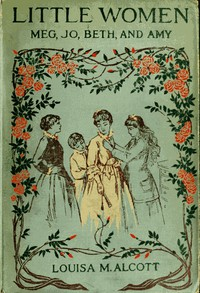
\includegraphics[width=0.25\columnwidth]{figures/pngs/little women cover.jpg}
\end{figure}

\begin{table}[h]
    \caption{Ranking the use of the most important \textsc{Children's} themes for \#1 downloaded \textsc{Children's} book, \textit{Little Women} relative to other \textsc{Children's} books in the dataset}
    \label{tab:little women}
    \begin{tabular}{l|r}
        \hline
        \centering
        \textsc{Theme} & \textsc{Rank} \\
        \hline
        Communication of Ideas & 2 \\
        Formation of Ideas & 2 \\
        Personal & 2 \\
        Moral & 3 \\
        Affections & 8 \\
        \hline
    \end{tabular}
\end{table}

Our Thematic observations hold true for each genre, but there is not one theme shared by all 12 genres.%, and Table~\ref{tab:theme counts} shows the distribution of Theme prioritization across all 12 genres.
This adheres to the observation we made about the WNRT and its lack of improvement after feature reduction for predicting success of all books.

\section{Experimental Results}\label{sec:experimental-results}

\subsection*{Classification Results}
The prediction accuracy for each model by genre, and each model across all books, both before and after feature reduction are shown in Table~\ref{tab:results by genre} and Table~\ref{tab:results all}, respectively\footnote{All WordNet to Roget models are mapped from WordNet\textsuperscript{R}}.
As illustrated in both settings, the performance of nearly every model improved after we reduced the features with WordNet showing the largest improvement of an average of 11.9\% when reduced by genre and 8.8\% when reduced independent of genre.

The best performing models are indicated in bold in Table~\ref{tab:results by genre} and Table~\ref{tab:results all}.
When predicting novel success by genre, WordNet\textsuperscript{R} and WNRC\textsuperscript{R} show the best results with both models predicting a book's success class at 95.4\%.
WordNet\textsuperscript{R} is most accurate with \textsc{Adventure} books, with an accuracy of 98.5\%, while WNRC\textsuperscript{R} is able to predict the success of \textsc{Historical Fiction} books with 100\% accuracy.
When predicting the success of a book independent of genre, WordNet\textsuperscript{R} remains the most accurate at 86.3\%.

Figure~\ref{fig:wn feature reduction} illustrates the pattern of performance improvement that each model exhibits through the feature reduction process both by genre and independent of genre.
As the number of features is reduced, the average accuracy for success prediction increases until the algorithm finds the best set of features and achieves peak performance.
Then accuracy sharply drops as the feature set is reduced further.
The fact that each model demonstrates such behavior validates the effectiveness of our feature reduction method.

\begin{table}[!t]
    \caption{Accuracy (\%) of classification results for all books, before/after feature reduction}
    \label{tab:results all}
    \begin{tabular}{c|c|c}
        % \hline
        \centering
        \textsc{Model} & \textsc{Accuracy} & \textsc{Accuracy\textsuperscript{R}} \\
        \hline
        Unigram & 68.7 & \textbf{70.3} \\
        % Unigram\textsuperscript{R} & 86.2}\\
        % \hline
        % Bigram & & & & & & & & & & & & & \\
        % Bigram\textsuperscript{R} & & & & & & & & & & & & & \\
        \hline
        POS & 67.4%42330 
        & 67.4%42332 \\
        \\
        % POS\textsuperscript{R} & 73.0} \\
        \hline
        Roget & 73.5 & 74.8 \\
        % Roget\textsuperscript{R} & 81.8} \\
        \hline
        WordNet & 74.9 & \textbf{86.3} \\
        % WordNet\textsuperscript{R} & 92.6} \\
        \hline
        WNRC & 76.4 & \textbf{77.4} \\
        \hline
        WNRT & 69.5 & 69.5 \\
        % \hline
        % \hline
        % Average & ? & ?} \\
        % Average\textsuperscript{R} & 83.4} \\
        % \hline
        % $\Gamma$ & & & & & & & & & & & & & \\
        % $\Gamma^R$ & & & & & & & & & & & & & \\
        % \hline
        % $\Gamma^G$ & & & & & & & & & & & & & \\
        % $\Gamma^{G^R}$ & & & & & & & & & & & & & \\
        % \hline
        % $\gamma$ & & & & & & & & & & & & & \\
        % $\gamma^R$ & & & & & & & & & & & & & \\
        % \hline
        % $\gamma^G$ & & & & & & & & & & & & & \\
        % $\gamma^{G^R}$ & & & & & & & & & & & & & \\
        \hline
    \end{tabular}
\end{table}

\subsection*{Interpreting Book Success}\label{subsec:int book success}
While our reduced WordNet model displays excellent performance in both test settings (by genre and independent of genre), the resulting feature sets are not self-explanatory.
In other words, the Synsets that the model deems most important do not necessarily highlight some interesting aspect of successful books, expected or otherwise.
This is where \textit{Roget's Thesaurus} proves most valuable.

We figured that if we looked up the Roget Theme of each WordNet Synset that we would find that the successful and unsuccessful books prioritize different Themes.
This was possible due to the similarity in the structure of WordNet and \textit{Roget's Thesaurus} as explained in the \textbf{Methodology} section above.
With this hypothesis in mind, we mapped the reduced WordNet model to a new Roget model by first looking up the Roget Category of each Synset from the reduced WordNet feature set, and then summing the frequencies in each group of Sysnets.
Then, as we did with each previous model, we reduced the new WordNet-to-Roget-Category (WNRC) model.
From the WNRC\textsuperscript{R} model we mapped again, this time from Roget Categories to the 23 Roget Themes, which produced the WordNet-to-Roget-Themes (WNRT) model.

We did not expect the performance of the WNRC model, since it was conceived strictly as an intermediary map between WordNet and Roget Themes. 
WNRC produced the highest baseline results of all the models used in our experiments with 89.5\% average accuracy by genre, and was able to perfectly predict the success classification of \textsc{Historical Fiction} novels.
Furthermore, WNRC\textsuperscript{R} accurately predicts success classification per genre at an average rate of 95.4\%, tying it with WordNet\textsuperscript{R} as the best performing models we tested.
What's impressive about the accuracy of WNRC\textsuperscript{R} when compared to that of WordNet\textsuperscript{R} is the large difference in number of features used in each model as shown in Table~\ref{tab:wn vs wnrc features}.

\begin{table}[t]
    \caption{Number of features before/after reduction for WordNet, WNRC, and WNRT}
    \label{tab:wn vs wnrc features}
    \begin{tabular}{l|r|r|r}
        % \hline
        % \multirow{2}{*}{Genre} & \multicolumn{3}{|c}{Number of Features} \\
        % \cline{2-4}
        % & WordNet & WNRC & WNRS \\
        % \hline
        %%
        %%%%
        % UPDATE ALL %%%
        %%%%
        \centering
        \textsc{Genre} & \textsc{WordNet} & \textsc{WNRC} & \textsc{WNRT} \\
        \hline
        Adventure & 36,390 & 425 & 22 \\
        Adventure\textsuperscript{R} & 540 & 149 & 17 \\
        \hline
        Children & 39,179 & 864 & 23 \\
        Children\textsuperscript{R} & 2,117 & 210 & 14 \\
        \hline
        Detective & 31,833 & 840 & 21 \\
        Detective\textsuperscript{R} & 1,670 & 272 & 9 \\
        \hline
        Drama & 33,718 & 812 & 23 \\
        Drama\textsuperscript{R} & 1,996 & 333 & 3 \\
        \hline
        Fantasy & 32,483 & 779 & 21 \\
        Fantasy\textsuperscript{R} & 1,665 & 192 & 12 \\
        \hline
        Fiction & 43,655 & 963 & 23 \\
        Fiction\textsuperscript{R} & 4,407 & 403 & 10 \\
        \hline
        Hist. Fict. & 36,902 & 815 & 22 \\
        Hist. Fict.\textsuperscript{R} & 864 & 198 & 14 \\
        \hline
        Humor & 37,457 & 822 & 22 \\
        Humor\textsuperscript{R} & 1,493 & 324 & 7 \\
        \hline
        Poetry & 38,412 & 872 & 23 \\
        Poetry\textsuperscript{R} & 3,004 & 243 & 7 \\
        \hline
        Romance & 36,137 & 451 & 23 \\
        Romance\textsuperscript{R} & 688 & 129 & 12 \\
        \hline
        Sci-Fi & 37,835 & 617 & 23 \\
        Sci-Fi\textsuperscript{R} & 1,190 & 225 & 6 \\
        \hline
        Short & 36,912 & 964 & 22 \\
        Short\textsuperscript{R} & 3,769 & 217 & 16 \\
        \hline
        All & 48,461 & 1,001 & 23 \\
        All\textsuperscript{R} & 7,415 & 374 & 23 \\
        \hline
    \end{tabular}
\end{table}

With such impressive results from WNRC\textsuperscript{R}, we expected WNRT and WNRT\textsuperscript{R} to follow suit despite learning with a feature set of at most 23 features.
WNRT\textsuperscript{R} achieves an average accuracy of 83.7\% learning from an average of only 10 features. 
While the performance of WNRT\textsuperscript{R} is impressive given the few number of features it requires, the purpose of WNRT\textsuperscript{R} was not to outperform WordNet\textsuperscript{R} or WNRC\textsuperscript{R}.
As previously state, the motivation for the construction of WNRT was strictly to find a common thread between successful novels in each genre.
That said, the decent performance of the WNRT\textsuperscript{R} model does support the reasoning behind its conception, and provide further evidence that WordNet\textsuperscript{R} and WNRC\textsuperscript{R} are general models that can reveal underlying characteristics of successful books.

\begin{table*}[!t]
    \caption{Top 5 most important themes for classifying \textsc{Children} novels and successful/unsuccessful thematic words}
    \label{tab:child themes}
    \begin{tabular}{l|ll}
        \hline
        \centering
        \multirow{2}{*}{\textsc{Theme}} & \multicolumn{2}{c}{\textsc{Words}} \\
        \cline{2-3}
        & \multicolumn{1}{c|}{Successful} & \multicolumn{1}{c}{Unsuccessful} \\
        \hline
        Affections & enthusiastic, lively, tenderness & inactive, sluggish, dull \\
        Communication of Ideas & secret, untruth, language & school, grammar, taciturnity \\
        Formation of Ideas & incredulity, impossibility, curiosity & dissent, sanity, memory \\
        Moral & gluttony, impurity, selfishness & punishment, virtue, duty \\
        Personal & expecting, blemish, hopelessness & aggravation, dejection, dullness \\
        \hline
    \end{tabular}
\end{table*}

Additionally, WNRT does not improve performance after feature reduction when classifying independent of genre.
This outcome also supports our original hypothesis as it shows that the model requires each of the 23 Roget Themes in order to make the most accurate prediction.
The lack of improvement in WNRT\textsuperscript{R} when predicting success class independent of genre also demonstrates the relationship between a novel's genre and its prioritization of certain Themes.

\subsection*{Successful Lexical Choices}\label{subsec:successful lexical choices}

After mapping the resulting feature weights of our WordNet\textsuperscript{R} model to Roget Themes, we were able to highlight the most important Themes when classifying the success of a novel given its genre.
Table~\ref{tab:child themes} gives the most important themes in predicting the success of \textsc{Children's} novels and the successful and unsuccessful semantic word groups within those themes.
These results clearly identify words associated with "school" and "grammar" as key contributors to unsuccessful \textsc{Children's} novels, while words like "secret," "enthusiastic," and "selfishness" contribute to successful \textsc{Children's} novels.

The indicated Themes align with intuitive expectations for \textsc{Children's} books, especially the presence of \textsc{Formation of Ideas} and \textsc{Moral}.
To verify these results, we looked at the most downloaded \textsc{Children's} book, \textit{Little Women}.
We ranked each book in the \textsc{Children's} genre according to the frequency of each prioritized Themes listed in Table~\ref{tab:little women}.
Then, we looked to see where \textit{Little Women} ranked for each of the Themes.
\textit{Little Women}'s use of the top Themes matches up as expected, as it ranks in the top three for four of the five most important Themes, and eighth for the fifth as shown in Table~\ref{tab:little women}.
The opposite is true for the least downloaded books, which all rank at the bottom for use of the most important Themes.

% \begin{figure}[t]
    \centering
    \caption{\textit{Little Women} by Louisa May Alcott}
    \label{fig:little women cover}
    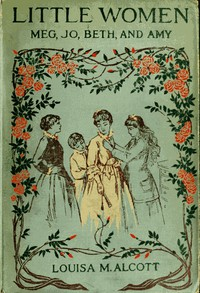
\includegraphics[width=0.25\columnwidth]{figures/pngs/little women cover.jpg}
\end{figure}

\begin{table}[h]
    \caption{Ranking the use of the most important \textsc{Children's} themes for \#1 downloaded \textsc{Children's} book, \textit{Little Women} relative to other \textsc{Children's} books in the dataset}
    \label{tab:little women}
    \begin{tabular}{l|r}
        \hline
        \centering
        \textsc{Theme} & \textsc{Rank} \\
        \hline
        Communication of Ideas & 2 \\
        Formation of Ideas & 2 \\
        Personal & 2 \\
        Moral & 3 \\
        Affections & 8 \\
        \hline
    \end{tabular}
\end{table}

Our Thematic observations hold true for each genre, but there is not one theme shared by all 12 genres.%, and Table~\ref{tab:theme counts} shows the distribution of Theme prioritization across all 12 genres.
This adheres to the observation we made about the WNRT and its lack of improvement after feature reduction for predicting success of all books.

% \begin{table*}[!t]
    \caption{Top 5 most important themes for classifying \textsc{Children} novels and successful/unsuccessful thematic words}
    \label{tab:child themes}
    \begin{tabular}{l|ll}
        \hline
        \centering
        \multirow{2}{*}{\textsc{Theme}} & \multicolumn{2}{c}{\textsc{Words}} \\
        \cline{2-3}
        & \multicolumn{1}{c|}{Successful} & \multicolumn{1}{c}{Unsuccessful} \\
        \hline
        Affections & enthusiastic, lively, tenderness & inactive, sluggish, dull \\
        Communication of Ideas & secret, untruth, language & school, grammar, taciturnity \\
        Formation of Ideas & incredulity, impossibility, curiosity & dissent, sanity, memory \\
        Moral & gluttony, impurity, selfishness & punishment, virtue, duty \\
        Personal & expecting, blemish, hopelessness & aggravation, dejection, dullness \\
        \hline
    \end{tabular}
\end{table*} % moved to results/main for spacing

\section{Future Work}\label{sec:future work}

The discoveries made in our research are just the beginning of what can be done with our dataset.
In addition to the data utilized for this project, we also extracted bi-gram and context-free grammar production features from each book.
In future work, we will continue to explore the impact of these features in addition to semantic word associations on book success.

We also believe that we could achieve better results through the use of a different success surrogate metric.
The scale of Project Gutenberg's catalog does not correspond to the website's popularity.
Therefore, as we continue this work we will include ratings from popular sites such as Goodreads.com, Amazon, etc. to acquire a even more accurate measurement of success~\cite{goodreads}.

\section{Conclusion}\label{sec:conclusion}

\subsection*{Classification Results}
The prediction accuracy for each model by genre, and each model across all books, both before and after feature reduction are shown in Table~\ref{tab:results by genre} and Table~\ref{tab:results all}, respectively\footnote{All WordNet to Roget models are mapped from WordNet\textsuperscript{R}}.
As illustrated in both settings, the performance of nearly every model improved after we reduced the features with WordNet showing the largest improvement of an average of 11.9\% when reduced by genre and 8.8\% when reduced independent of genre.

The best performing models are indicated in bold in Table~\ref{tab:results by genre} and Table~\ref{tab:results all}.
When predicting novel success by genre, WordNet\textsuperscript{R} and WNRC\textsuperscript{R} show the best results with both models predicting a book's success class at 95.4\%.
WordNet\textsuperscript{R} is most accurate with \textsc{Adventure} books, with an accuracy of 98.5\%, while WNRC\textsuperscript{R} is able to predict the success of \textsc{Historical Fiction} books with 100\% accuracy.
When predicting the success of a book independent of genre, WordNet\textsuperscript{R} remains the most accurate at 86.3\%.

Figure~\ref{fig:wn feature reduction} illustrates the pattern of performance improvement that each model exhibits through the feature reduction process both by genre and independent of genre.
As the number of features is reduced, the average accuracy for success prediction increases until the algorithm finds the best set of features and achieves peak performance.
Then accuracy sharply drops as the feature set is reduced further.
The fact that each model demonstrates such behavior validates the effectiveness of our feature reduction method.

\begin{table}[!t]
    \caption{Accuracy (\%) of classification results for all books, before/after feature reduction}
    \label{tab:results all}
    \begin{tabular}{c|c|c}
        % \hline
        \centering
        \textsc{Model} & \textsc{Accuracy} & \textsc{Accuracy\textsuperscript{R}} \\
        \hline
        Unigram & 68.7 & \textbf{70.3} \\
        % Unigram\textsuperscript{R} & 86.2}\\
        % \hline
        % Bigram & & & & & & & & & & & & & \\
        % Bigram\textsuperscript{R} & & & & & & & & & & & & & \\
        \hline
        POS & 67.4%42330 
        & 67.4%42332 \\
        \\
        % POS\textsuperscript{R} & 73.0} \\
        \hline
        Roget & 73.5 & 74.8 \\
        % Roget\textsuperscript{R} & 81.8} \\
        \hline
        WordNet & 74.9 & \textbf{86.3} \\
        % WordNet\textsuperscript{R} & 92.6} \\
        \hline
        WNRC & 76.4 & \textbf{77.4} \\
        \hline
        WNRT & 69.5 & 69.5 \\
        % \hline
        % \hline
        % Average & ? & ?} \\
        % Average\textsuperscript{R} & 83.4} \\
        % \hline
        % $\Gamma$ & & & & & & & & & & & & & \\
        % $\Gamma^R$ & & & & & & & & & & & & & \\
        % \hline
        % $\Gamma^G$ & & & & & & & & & & & & & \\
        % $\Gamma^{G^R}$ & & & & & & & & & & & & & \\
        % \hline
        % $\gamma$ & & & & & & & & & & & & & \\
        % $\gamma^R$ & & & & & & & & & & & & & \\
        % \hline
        % $\gamma^G$ & & & & & & & & & & & & & \\
        % $\gamma^{G^R}$ & & & & & & & & & & & & & \\
        \hline
    \end{tabular}
\end{table}

\subsection*{Interpreting Book Success}\label{subsec:int book success}
While our reduced WordNet model displays excellent performance in both test settings (by genre and independent of genre), the resulting feature sets are not self-explanatory.
In other words, the Synsets that the model deems most important do not necessarily highlight some interesting aspect of successful books, expected or otherwise.
This is where \textit{Roget's Thesaurus} proves most valuable.

We figured that if we looked up the Roget Theme of each WordNet Synset that we would find that the successful and unsuccessful books prioritize different Themes.
This was possible due to the similarity in the structure of WordNet and \textit{Roget's Thesaurus} as explained in the \textbf{Methodology} section above.
With this hypothesis in mind, we mapped the reduced WordNet model to a new Roget model by first looking up the Roget Category of each Synset from the reduced WordNet feature set, and then summing the frequencies in each group of Sysnets.
Then, as we did with each previous model, we reduced the new WordNet-to-Roget-Category (WNRC) model.
From the WNRC\textsuperscript{R} model we mapped again, this time from Roget Categories to the 23 Roget Themes, which produced the WordNet-to-Roget-Themes (WNRT) model.

We did not expect the performance of the WNRC model, since it was conceived strictly as an intermediary map between WordNet and Roget Themes. 
WNRC produced the highest baseline results of all the models used in our experiments with 89.5\% average accuracy by genre, and was able to perfectly predict the success classification of \textsc{Historical Fiction} novels.
Furthermore, WNRC\textsuperscript{R} accurately predicts success classification per genre at an average rate of 95.4\%, tying it with WordNet\textsuperscript{R} as the best performing models we tested.
What's impressive about the accuracy of WNRC\textsuperscript{R} when compared to that of WordNet\textsuperscript{R} is the large difference in number of features used in each model as shown in Table~\ref{tab:wn vs wnrc features}.

\begin{table}[t]
    \caption{Number of features before/after reduction for WordNet, WNRC, and WNRT}
    \label{tab:wn vs wnrc features}
    \begin{tabular}{l|r|r|r}
        % \hline
        % \multirow{2}{*}{Genre} & \multicolumn{3}{|c}{Number of Features} \\
        % \cline{2-4}
        % & WordNet & WNRC & WNRS \\
        % \hline
        %%
        %%%%
        % UPDATE ALL %%%
        %%%%
        \centering
        \textsc{Genre} & \textsc{WordNet} & \textsc{WNRC} & \textsc{WNRT} \\
        \hline
        Adventure & 36,390 & 425 & 22 \\
        Adventure\textsuperscript{R} & 540 & 149 & 17 \\
        \hline
        Children & 39,179 & 864 & 23 \\
        Children\textsuperscript{R} & 2,117 & 210 & 14 \\
        \hline
        Detective & 31,833 & 840 & 21 \\
        Detective\textsuperscript{R} & 1,670 & 272 & 9 \\
        \hline
        Drama & 33,718 & 812 & 23 \\
        Drama\textsuperscript{R} & 1,996 & 333 & 3 \\
        \hline
        Fantasy & 32,483 & 779 & 21 \\
        Fantasy\textsuperscript{R} & 1,665 & 192 & 12 \\
        \hline
        Fiction & 43,655 & 963 & 23 \\
        Fiction\textsuperscript{R} & 4,407 & 403 & 10 \\
        \hline
        Hist. Fict. & 36,902 & 815 & 22 \\
        Hist. Fict.\textsuperscript{R} & 864 & 198 & 14 \\
        \hline
        Humor & 37,457 & 822 & 22 \\
        Humor\textsuperscript{R} & 1,493 & 324 & 7 \\
        \hline
        Poetry & 38,412 & 872 & 23 \\
        Poetry\textsuperscript{R} & 3,004 & 243 & 7 \\
        \hline
        Romance & 36,137 & 451 & 23 \\
        Romance\textsuperscript{R} & 688 & 129 & 12 \\
        \hline
        Sci-Fi & 37,835 & 617 & 23 \\
        Sci-Fi\textsuperscript{R} & 1,190 & 225 & 6 \\
        \hline
        Short & 36,912 & 964 & 22 \\
        Short\textsuperscript{R} & 3,769 & 217 & 16 \\
        \hline
        All & 48,461 & 1,001 & 23 \\
        All\textsuperscript{R} & 7,415 & 374 & 23 \\
        \hline
    \end{tabular}
\end{table}

With such impressive results from WNRC\textsuperscript{R}, we expected WNRT and WNRT\textsuperscript{R} to follow suit despite learning with a feature set of at most 23 features.
WNRT\textsuperscript{R} achieves an average accuracy of 83.7\% learning from an average of only 10 features. 
While the performance of WNRT\textsuperscript{R} is impressive given the few number of features it requires, the purpose of WNRT\textsuperscript{R} was not to outperform WordNet\textsuperscript{R} or WNRC\textsuperscript{R}.
As previously state, the motivation for the construction of WNRT was strictly to find a common thread between successful novels in each genre.
That said, the decent performance of the WNRT\textsuperscript{R} model does support the reasoning behind its conception, and provide further evidence that WordNet\textsuperscript{R} and WNRC\textsuperscript{R} are general models that can reveal underlying characteristics of successful books.

\begin{table*}[!t]
    \caption{Top 5 most important themes for classifying \textsc{Children} novels and successful/unsuccessful thematic words}
    \label{tab:child themes}
    \begin{tabular}{l|ll}
        \hline
        \centering
        \multirow{2}{*}{\textsc{Theme}} & \multicolumn{2}{c}{\textsc{Words}} \\
        \cline{2-3}
        & \multicolumn{1}{c|}{Successful} & \multicolumn{1}{c}{Unsuccessful} \\
        \hline
        Affections & enthusiastic, lively, tenderness & inactive, sluggish, dull \\
        Communication of Ideas & secret, untruth, language & school, grammar, taciturnity \\
        Formation of Ideas & incredulity, impossibility, curiosity & dissent, sanity, memory \\
        Moral & gluttony, impurity, selfishness & punishment, virtue, duty \\
        Personal & expecting, blemish, hopelessness & aggravation, dejection, dullness \\
        \hline
    \end{tabular}
\end{table*}

Additionally, WNRT does not improve performance after feature reduction when classifying independent of genre.
This outcome also supports our original hypothesis as it shows that the model requires each of the 23 Roget Themes in order to make the most accurate prediction.
The lack of improvement in WNRT\textsuperscript{R} when predicting success class independent of genre also demonstrates the relationship between a novel's genre and its prioritization of certain Themes.

\subsection*{Successful Lexical Choices}\label{subsec:successful lexical choices}

After mapping the resulting feature weights of our WordNet\textsuperscript{R} model to Roget Themes, we were able to highlight the most important Themes when classifying the success of a novel given its genre.
Table~\ref{tab:child themes} gives the most important themes in predicting the success of \textsc{Children's} novels and the successful and unsuccessful semantic word groups within those themes.
These results clearly identify words associated with "school" and "grammar" as key contributors to unsuccessful \textsc{Children's} novels, while words like "secret," "enthusiastic," and "selfishness" contribute to successful \textsc{Children's} novels.

The indicated Themes align with intuitive expectations for \textsc{Children's} books, especially the presence of \textsc{Formation of Ideas} and \textsc{Moral}.
To verify these results, we looked at the most downloaded \textsc{Children's} book, \textit{Little Women}.
We ranked each book in the \textsc{Children's} genre according to the frequency of each prioritized Themes listed in Table~\ref{tab:little women}.
Then, we looked to see where \textit{Little Women} ranked for each of the Themes.
\textit{Little Women}'s use of the top Themes matches up as expected, as it ranks in the top three for four of the five most important Themes, and eighth for the fifth as shown in Table~\ref{tab:little women}.
The opposite is true for the least downloaded books, which all rank at the bottom for use of the most important Themes.

% \begin{figure}[t]
    \centering
    \caption{\textit{Little Women} by Louisa May Alcott}
    \label{fig:little women cover}
    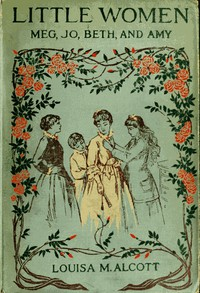
\includegraphics[width=0.25\columnwidth]{figures/pngs/little women cover.jpg}
\end{figure}

\begin{table}[h]
    \caption{Ranking the use of the most important \textsc{Children's} themes for \#1 downloaded \textsc{Children's} book, \textit{Little Women} relative to other \textsc{Children's} books in the dataset}
    \label{tab:little women}
    \begin{tabular}{l|r}
        \hline
        \centering
        \textsc{Theme} & \textsc{Rank} \\
        \hline
        Communication of Ideas & 2 \\
        Formation of Ideas & 2 \\
        Personal & 2 \\
        Moral & 3 \\
        Affections & 8 \\
        \hline
    \end{tabular}
\end{table}

Our Thematic observations hold true for each genre, but there is not one theme shared by all 12 genres.%, and Table~\ref{tab:theme counts} shows the distribution of Theme prioritization across all 12 genres.
This adheres to the observation we made about the WNRT and its lack of improvement after feature reduction for predicting success of all books.

\bibliographystyle{ACM-Reference-Format}
\bibliography{ref}

\end{document}
